\documentclass[10pt]{article}


\usepackage{lipsum}
\usepackage{graphicx}
\usepackage{amsmath}
\usepackage{hyperref}

\usepackage[section]{placeins}

\usepackage{etoolbox}
\usepackage[onehalfspacing]{setspace}
\AtBeginEnvironment{figure}{\singlespacing}
\AtBeginEnvironment{table}{\singlespacing}

\usepackage{caption}
\DeclareCaptionFont{8pt}{\fontsize{8pt}{9pt}\selectfont}
\captionsetup{font={8pt}}
\usepackage{todonotes}
%\usepackage[disable]{todonotes}

\usepackage[
	backend=biber,
    style=authoryear,
	url=false,
    %sorting=ynt,
    bibwarn=true,
    bibencoding=utf8,
	uniquename=false,
	uniquelist=false,
    sortlocale=de_DE,
    maxbibnames=99,
    maxcitenames=2]{biblatex}
\renewbibmacro{in:}{}
    
\DefineBibliographyStrings{english}{
   andothers = {{et\,al\adddot}},}
   
\addbibresource{../../../bib/thesis.bib}
\AtEveryBibitem{\clearfield{month}}
\AtEveryCitekey{\clearfield{month}}

\AtBeginEnvironment{figure}{\singlespacing}
\AtBeginEnvironment{table}{\singlespacing}


\begin{document}
%\the\textwidth 
%\makeatletter\f@size
% 345 pt = 4.79167 in -> figures 4.75 in 
% text 10 pt, fig caption 8 pt
% in drawio 10 pt -> 13.3; 8 pt -> 10.66 

\begin{titlepage}
	\centering
	{\scshape\LARGE Ludwig-Maximilians-Universität München \par}
	{\scshape\large Faculty of Biology, Computational Neuroscience \par}
	\vspace{0.7cm}
	\includegraphics[width=0.3\textwidth]{../logo/siegel_black.pdf}\par
	\includegraphics[width=0.7\textwidth]{../logo/GSN-Logo_ab35mmBreite_RGB.jpg}\par
	\vspace{0.5cm}

	{\scshape\LARGE Master's Thesis}
	\rule{\textwidth}{1.pt}
	{\huge\bfseries Computational Simulation of Time Perception \par}
	\rule{\textwidth}{1.pt}
	\vspace{0.5cm}

	{\Large Katharina \textsc{M Bracher} \par}
	%{Student ID: 11754625 \par}
	\vspace{0.7cm}

	{\large Supervision: Dr. Kay \textsc{Thurley} \par}
	{\large Prof. Dr. Andreas \textsc{Herz} \par}
\end{titlepage}


\normalsize

\section*{Abstract}

% Background brain
Timing in the brain is thought to be encoded through population state dynamics of neurons.
Experimentally, reproduction tasks are a useful approach to study sensory processing pf time because a relationship between external events and their internal perception is established.
In such experiments, behavioral responses are characterized by specific biases such as the central tendency or regression effect, i.e. the overestimation of small time intervals and the underestimation of large ones.
How this is implemented, however, remains unknown.
Here I investigate a neural circuit model that has been proposed recently to explain various timing behaviors, and apply it to realistic time reproduction experiments.  Parameters that yield minimal error in behavior predict the characteristic behavioral effects. 

Using these parameters, I further investigate the effects of stimulus statistics on the behavior and found that the model predicts no influence of stimulus variance on behavior. 
These results are partially confirmed in gerbil data, suggesting an adjustment to accommodate stimulus statistics leads to better performance in cases of high variance. 
This work provides further evidence that a dynamical systems perspective has the potential to explain flexible timing.


%Robust conditions for were identified that are consistent with the key behavioral effects. 
%Increasing evidence suggests, that the brain encodes time in population state dynamics. 
%In order to flexibly adjust behavior, the brain is thought to dynamically change these patterns of neural activity.
%A crucial parameter is the weight with which error signal is weighted to update 
%Adjusting this weight in accordance with error minimization, leads to putting more weight on the prior experience for longer stimuli, which naturally entail more uncertainty, and is thus biological plausible.
%The model makes use of a predictive coding mechanism and adjusts the speed of a readout unit according to an error signal.
%In the dynamical systems approach, adjusting the initial conditions and external inputs to the system leads to control of population dynamics.
%The speed of neural dynamics is adjusted according to the reproduced time interval.
%Humans and animals are able to flexibly coordinate and anticipate behaviors. 
%Sensory information is combined expectations based on prior knowledge to minimize errors arising from noise in the environment and neural signal. 

\pagebreak

\tableofcontents

\pagebreak

\section{Introduction}
Animals are capable of producing complex and flexible behaviors that rely on the interplay of motor and sensory systems.
Timing is critical for many of these sensorimotor functions, ensuring the ability to anticipate and coordinate interactions with the environment.
Sensory and motor timing in the millisecond range is particularly important, as this timescale includes temporal cues for vocalization as well as fine motor coordination.
Despite its importance, there is no sensory organ responsible for time perception, which means that perception must be generated internally by extracting information from sensory inputs.
Although time is pervasive in animal behavior, it is elusive and difficult to study. The neural implementation that allows the brain to perceive and internally perform complex temporal computations remains unknown.
Nevertheless, the mechanism of timing might provide powerful insights into general mechanisms of cognition and neural computations (\cite{Issa2020}).

Magnitude estimation is a useful approach to explore sensory processing because it involves establishing a relationship between external events and their internal perception by, for example, evaluating or reproducing a time interval. 
However, externally-derived inputs are subject to noise arising from the variability of the environment. In addition, noise arising from neural representations of the input affects the perception.
A variety of experimental studies have found characteristic behavioral effects in magnitude estimation that might arise to minimize errors in the presence of noise (\cite{Petzschner2015}).

In the following, key effects of magnitude estimation are discussed. I then summarize evidence for brain dynamics underlying time perception and introduce a model that I use in this work to simulate time perception.

\subsection{Behavioral Effects in Magnitude Estimation}
%---> magnitude estimation, optimization, Bayes
Magnitude estimation exhibits characteristic effects across sensory modalities.
The most striking observation is regression to the mean of stimuli, in other words, small stimuli are overestimated whereas large stimuli are underestimated (\textit{regression effect}). 
This effect intensifies for ranges with larger stimuli (\textit{range effect}).
Also, the standard deviation of estimates increases monotonically for larger stimuli (\textit{scalar variability}). 
Finally, the recent history of stimuli presentations influences the current stimuli estimation (\textit{sequential effects}).
All effects mentioned above are displayed in Fig. \ref{fig:behavioraleffects}. 
Modality-independence of these effects suggests the existence of a common underlying principle or processing mechanisms, that would explain e.g. an optimal strategy for unreliable judgments due to noise.
Minimizing errors in judgment can be achieved by integrating prior experience with immediate sensory input, and is therefore often described with Bayesian models.
In Bayesian models, sensory information is represented by a likelihood function and is combined with prior experience that together result in biased estimates (\cite{Knill2004}). 
Ongoing research is trying to identify mechanisms of how the brain would implement such behavior. %a bayesian framework?; 
\todo{However, is has not been shown how the brain would implement such behavior. -- Why not? I guess people have tried to. Either forward reference of give a short intuition.}

\begin{figure}[ht]
	\centering
	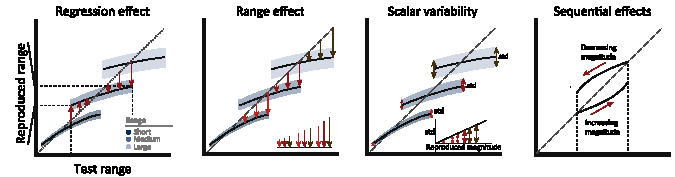
\includegraphics[width=\textwidth]{figures/behavioural_effects_petzschner.pdf}
	\caption{\textbf{Behavioral effects.} 
	\textit{Regression effect}: in a distribution of stimuli large stimuli are underestimated, and small stimuli are overestimated which results in a regression to the mean of the range.
	\textit{Range effect}: the regression to the mean gets more pronounced for ranges that comprise larger stimuli. 
	\textit{Scalar variability}: the standard deviation of the reproduced magnitude grows linearly with larger estimates. 
	\textit{Sequential effects}: the history of presented stimuli (e.g. ascending or descending order) has an influence on the reproduced magnitude. 
	(Adapted from \cite{Petzschner2015}, reproduced with permission from F. Petzschner.)}
	\label{fig:behavioraleffects}
\end{figure}

\subsection{Time Estimation via Predictive Timing}
%---> timing, time reproduction experiments, methods to measure time 
Experiments, in which subjects have to measure and reproduce time intervals, allow us to study how the brain integrates expectations with current sensory input in order to achieve correct timing.
Time reproduction is usually accomplished by at least one presentation of the time interval e.g. between two external events (sensory timing), and a reproduction period that is indicated by the subject's response (motor timing).
In both epochs elapsed time needs to be estimated, the difference lies in the termination of the interval. In sensory timing, the time interval is terminated by an external event, while in motor timing, the completion is internally generated and executed by the subject's response (\cite{Grondin2010}).

Time between two events can be measured in an absolute or predictive manner. 
In the case of absolute timing, time can be continuously estimated from an output that results from integration of ticks from a central clock (\cite{Buhusi2005}, \cite{Paton2018}).
The rate at which activity increases does not depend on the time interval.
In contrast, for predictive timing a fixed state is reached at the end of the time interval, by adjusting the rate of a process according to the anticipated time.
Recently, evidence of predictive timing has emerged suggesting, that the central nervous system makes use of predictive signaling mechanisms, allowing the animal to contemplate sensory consequences of actions (\cite{Egger2019}, \cite{Meirhaeghe2021}).

Predictive coding is a framework, in which the brain is predicting its upcoming states and refining these predictions through error signals (\cite{Rao1999}, \cite{Huang2011}, \cite{Ficco2021}).
Intrinsic neural representations of motor actions are used as predictor of sensory consequences. % representations (efference copy)
If there is a mismatch in predicted and actual sensory feedback, an internal model is updated by the error signal (\cite{Bubic2010}, \cite{Clark2013}, \cite{Straka2018}). %mismatch (corollory discharge)  actual sensory feedback (reafference)
The internal model can include a prior to integrate expectations into the time estimate.
Based on predictions and expectations, flexible control of neural mechanisms is required to measure and produce time intervals.
This raises the question of how flexible control over brain dynamics can be achieved.

% Accordingly, the CNS needs to exert control and prediction to achieve desired or expected sensory consequences.
% the brain makes sense of the environment by predicting future events and by testing whether these are in line with incoming sensory information and previous experiences

\subsection{Brain Dynamics Underlying Time Perception}
%---> nerual implementation, brain ares, scaling, trajectories, speed command, motor simulationk error signal
Increasing evidence suggests, that the brain encodes time in population state dynamics. 
A brain area that has been associated with timing behavior is the frontal (\cite{Shima2000}, \cite{Lewis2004}, \cite{Genovesio2006}, \cite{Emmons2017}, \cite{Wang2018}).
In time reproduction experiments, the activity of individual cells in the frontal cortex heterogeneous response profiles, many of which are temporally scaled according to the produced time interval (\cite{Remington2018}, \cite{Wang2018}, \cite{Sohn2019}, \cite{Henke2021}).
Indeed, time can be encoded predictively relative to the mean of time intervals by temporal scaling activity.
Scaling is a phenomenon that is consistent at the population level, when activity is displayed in a low-dimensional state space. In the state space, the activity of all neurons is represented over time by a so-called neural trajectory (\cite{Cueva2022}).
It has been shown that for sensory timing, the population activity evolves along a common trajectory, whereas in motor timing, trajectories scale in speed to reach a common terminal state, that triggers an action (\cite{Mita2009}, \cite{Murakami2014}, \cite{Wang2018}, \cite{Sohn2019}, \cite{Henke2021}, \cite{Meirhaeghe2021}).
%In this case speed of the neural trajectory is inversely proportional to the time interval that is reproduced, thus scaled by the stimulus time interval
Experiments have shown a causal link for population dynamics encoding time. Cooling the  medial prefrontal cortex in rats, slowed population dynamics down, resulting in longer time estimates (\cite{Xu2014}). 
Therefore, the brain dynamically changes patterns of neural activity to flexibly adjust behavior to time actions, where flexible motor timing can be achieved by controlling the speed of neural dynamics (\cite{Remington2018}, \cite{Wang2018}, \cite{Sohn2019}, \cite{Tsao2022}).

\paragraph{A Circuit Model for Time Estimation.}
Data indicates that neural trajectories reflect the internal estimate of a time interval and are influenced by a prior.
Experiments with multiple, consecutive measurement periods showed a sequential update of the estimate, providing evidence for a predictive process with an error signal extracted from the previous epoch to correct the speed of the neural trajectory.
\citeauthor{Wang2018} (\citeyear{Wang2018}) proposed a potential neural mechanism for speed control by flexibly adjusting the effective time constant of a network.
In fact, the population activity reflects an interval-dependent speed command that is updated based on a mismatch between predicted and actual interval in measurement epochs (\cite{Wang2018}, \cite{Egger2019}). 

%---> Curcuit model, decision making, elements
%model used only for... in secific task
%Here, I aimed to answer this question using a dynamical systems approach. 

Building on these findings, \citeauthor{Remington2018} (\citeyear{Remington2018}) showed that flexible control of behavior in interval reproduction can be understood in terms of a dynamical system that is characterized by the initial state and an external input.
 In a two-neuron-model, which is well known for modeling decision-making (\cite{Wang2002}, \cite{Roxin2008}), the input level can be used to adapt the effective time constant of the system.
Based on that mechanism, \citeauthor{Egger2020} (\citeyear{Egger2020}) developed an extended circuit model for sensorimotor timing.
The model was used in interval reproduction tasks and fitted to human data that exhibited classical effects of magnitude estimation. 
However, different time intervals were presented separately and not in a random sequence as in classical time reproduction experiments. 
%This way expectations of the presented time intervals emerge over the course of the experiment.


\paragraph{Research Questions.}
By applying the circuit model to simulations that reflect more realistic conditions of time reproduction experiments, the present work addresses the question of which behavioral effects can be explained by the model. 
I demonstrate that in realistic experiment simulations, classical effects of magnitude estimation are reproduced by the model with parameters that minimize errors in behavior, providing further evidence that a dynamical systems perspective has the potential to explain flexible timing.
%, that itself is only based on principles found in brain data.
Following this result, I ask what effect external variability in time intervals has on behavior. 

In the subsequent two sections, the circuit model is described in detail. 
I discuss different input regimes of the model and identify model parameters that minimize errors in the behavior. 
In Section 4, I examine the behavior of the model and make adjustments to the experiment design to then investigate the effects of stimulus statistics on behavior in section 5. Furthermore, the predictions of the model are evaluated and compared to data of time reproduction experiments with gerbils and humans.

\section{A Circuit Model for Time Estimation}
The model is build on a basic circuit, which is introduced at the beginning. I then describe the extension of the circuit to include a mechanism for updating the external input (\cite{Egger2020}).
Depending on the input strength, the model operates in different regimes. 
In this section we focus on the intermediate input regime, but I will discuss the high input regime in Section 3.

\subsection{Basic Circuit}
Flexible speed control can be achieved by a model consisting only of three units, $u, v, y$ that represent population activity.
The dynamics of $u, v$, and $y$ are defined as follows:
\begin{equation} \label{circuit}
	\begin{split}
	\tau\frac{\text{d}u}{\text{d}t} & = -u + \theta(W_{uI}I - W_{uv}v + \eta_u) \;, \\
	\tau\frac{\text{d}v}{\text{d}t} & = -v + \theta(W_{vI}I - W_{vu}v + \eta_v) \;, \\
	\tau\frac{\text{d}y}{\text{d}t} & = -y + W_{yu}u - W_{yv}v + \eta_y \;.
	\end{split}
\end{equation}
Two units, $u$ and $v$, receive a tonic symmetric input $I$ ($W_{uI}=W_{vI}=6$) and are mutually inhibiting each other ($W_{uv}=W_{vu}=6$). 
The inputs to $u$ and $v$ are governed by a sigmoid activation function $\theta(x) = \frac{1}{1+\exp(-x)}$.
The output unit $y$ receives excitatory input from $u$ and inhibitory input from $v$ ($W_{yu}=W_{yv}=1$) which results in a ramp-like activity of $y$ (Fig. \ref{fig:circuit}a).
Different external inputs to the sigmoid activation function, control the effective time constants of the system. Stronger inputs drive the activation more towards the saturating nonlinearity, which leads to larger effective time constants.
Because of this, the model yields a repertoire of slopes that can be exploited for time reproduction (Fig. \ref{fig:circuit}c)(\cite{Egger2020}). 
Stochastic synaptic inputs are modeled as independent white noise $\eta_u, \eta_v, \eta_y$ with standard deviation $\sigma$.
%Noise is independently sampled for every time step from a Gaussian distribution with standard deviation $\sigma$.
To simulate the dynamics of $u, v, y$ and $I$, Euler's method was used with a step size $\Delta t$ that corresponds to 10 ms.
Depending on the input $I$, the system shows different dynamics.

\paragraph{The model has three distinct input regimes.}
For low levels of~$I$ (0~$<I<$~0.5) the system has three fixed points (two stable, one unstable at $u=v$) and $y$ ramps up faster the higher input~$I$. 
For intermediate values of $I$~(0.5~$<I<$~1) the system still shows three fixed points of the same sort as in the low input regime (Fig. \ref{fig:circuit}b) but $y$ ramps up with a slope that is inversely proportional to the input $I$ ($y$ ramps up slower the higher input $I$, cf. Fig. \ref{fig:circuit}c). 
For high $I$ (1~$<I$) the system has only one, but stable fixed point (at $u=v$), and $y$ ramps down faster for higher $I$.
Thus, the speed at which the output $y$ evolves can be controlled by the input $I$ (Fig. \ref{fig:circuit}d) and determines the time interval after which $y$ reaches a fixed threshold $y_{\text{th}}$. 
In interval reproduction experiments, reaching a threshold $y_{\text{th}}$ can be understood as movement initiation time, which can be controlled for by adjusting $I$.
In this section, the intermediate input regime is explored: higher inputs result in a shallower slope of $y$, such that the threshold $y_{\text{th}}$ is reached after a longer time interval.

%%%%%%%%%%%%%%%%%%%%%%%%%%%%%%%%%%%%%%%%%%%%%%%%%%%%%%%%%%%%%%%%%%%% nullcline
\begin{figure}[ht]
	\centering
	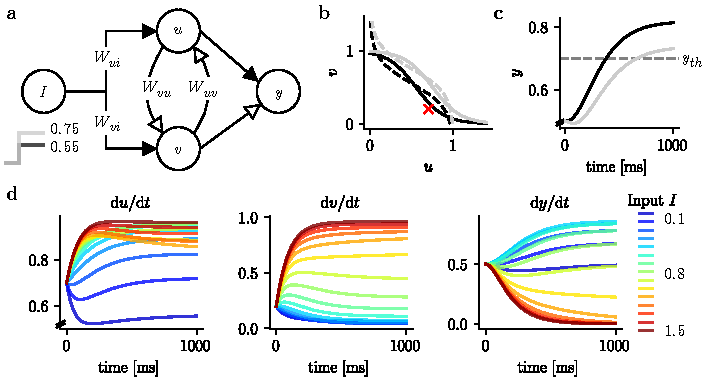
\includegraphics{figures/defCircuit_nullcl.pdf}
	\caption{\textbf{Basic circuit and input regimes.} 
	\textbf{(a)} $u$ and $v$ share a common input $I$. The input is governed by weights $W_{uI}$ and $W_{vI}$. The two units have reciprocal inhibitory connections, with weights $W_{uv}$ and $W_{vu}$ that determine the inhibitory strength. Both project to the output unit $y$ with an excitatory connection from $u$ and an inhibitory connection from $v$. Excitatory and inhibitory connections are shown by filled and open arrows, respectively. 
	\textbf{(b)} The control of the speed in $y$ can be analyzed in the phase plane of $u$ and $v$. The $u$ (dashed) and $v$ nullcline (solid) is shifted when the input is increased from $I=0.65$ (black) to $I=0.75$ (gray). In the intermediate regime, the system shows two stable and one unstable fixed point. The red cross indicates the initial conditions for the dynamics in (c). Depending on $I$, with the same initial conditions, the system evolves faster or slower to the stable fixed point. 
	\textbf{(c)} Dynamics of $y$ for intermediate regime with input $I=0.75$ in gray and $I=0.65$ in black. There is an inverse relation of input strength and slope. With higher input, the threshold at 0.7 (dashed line) is reached after a longer time interval. 
	\textbf{(d)} Dynamics of $u, v, y$ for inputs from $0.1\leq I \leq 1.5$ are shown. Initial conditions are set to $u_0=0.7, v_0=0.2, y_0=0.5$. With these initial conditions and values of $I>=0.5$, the relation of steady state activity of $y$ (and slope to reach the steady state) is inverse to $I$ (intermediate and high $I$ regime). For values $I<=1$ the activity of $y$ ramps down (yellow corresponds to $I=1$). For $I<0.5$ the steady state (slope) is smaller the smaller $I$ (low $I$ regime, dark blue).}
\label{fig:circuit}
\end{figure}

\subsection{Extended Circuit for Experiment Simulation} %Update Mechanism and Experiment Procedure
Basic interval reproduction experiments can be designed with only two epochs: a measurement epoch that has the duration of the stimulus interval and a reproduction epoch that starts immediately after the measurement epoch (Fig. \ref{fig:epochs}b). Typically, a delay is introduced between subsequent trials. 
The basic circuit described above is modified to perform interval reproduction (cf. Figure \ref{fig:epochs}a for schematic of the modified circuit).
To achieve time reproduction, the relation of input $I$ with the slope of the ramping activity of $y$ is used in combination with a fixed threshold $y_{\text{th}}$.
By introducing an update mechanism that flexibly adjusts $I$, the threshold crossing of $y$ can be delayed or moved to earlier times.
This way, measuring and reproducing an interval is done predictively, by adjusting the slope of the ramp such that the output reaches the threshold after the intended time.
%In other scenarios, time could be encoded by the level a ramp reaches with a fixed slope.
In the model, the measurement epoch is specified by the stimulus interval $t_s$, whereas the reproduction ends when $y$ reaches the fixed threshold $y_{\text{th}}$ from below. 
The time from the end of the measurement epoch until the threshold-crossing of $y$ yields the reproduced time interval $t_r$ that is aimed to equal the stimulus interval $t_s$ (Fig. \ref{fig:epochs}c).

\begin{figure}
	\centering
	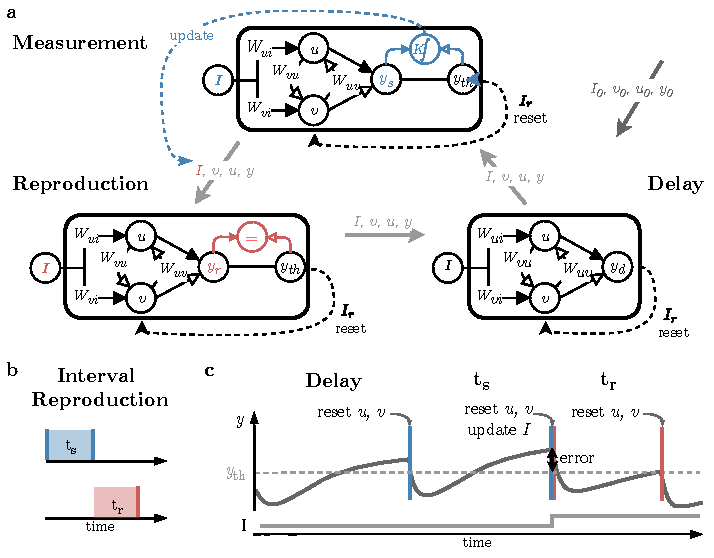
\includegraphics{figures/epochs.pdf}
	\caption{\textbf{Extended circuit for experiment simulation.} 
	\textbf{(a)} The circuits for measurement, reproduction and delay epoch are displayed. All circuits comprise the same basic structure with different additional elements that are unique for the epoch. Initial values of $u, v, y$ and $I$ are fed into the delay circuit for the duration of the initial interval. $u$ and $v$ are reset with a transient input $I_r$ before end values of $u, v, y$ and $I$ are transferred to the measurement circuit as new initial conditions. After the duration of the stimulus interval, the difference between $y$ and the threshold $y_{\text{th}}$ is used with the memory parameter $K$ to update $I$ together with another reset of $u$ and $v$. The values are transferred with all other variables to the reproduction circuit. The reproduction epoch ends when $y$ reaches the threshold $y_{\text{th}}$ from below. Before the presentation of another stimulus interval, there is again a delay period with no update of $I$. The reset mechanism enables the model to simulate an arbitrary number of stimulus intervals. Adapted from \cite{Egger2020}.
	\textbf{(b)} Interval reproduction experiment with stimulus interval $t_s$ (blue) and reproduction $t_r$ (red).
	\textbf{(c)} Schematic of one trial. After a delay epoch, $u$ and $v$ are reset. The measurement epoch lasts for the duration of the stimulus interval $t_s$. $y$ should reach the threshold $y_{\text{th}}$ (dashed line) at exactly the time the stimulus interval ends. The threshold was crossed well before the end of the interval and at the end of the measurement epoch, the error in $y_m$ to the threshold $y_{\text{th}}$ is used to update $I$. To reach the threshold at a later time, $I$ is increased, which reduces the slope of $y$ in the reproduction epoch. After the reset of $u$ and $y$ and the update of $I$ the reproduction ends when $y$ reaches the threshold. The time after the reset and update until the threshold crossing denotes the reproduced interval $t_r$.}
\label{fig:epochs}
\end{figure}

\paragraph{An update mechanism adjusts the input for reproductions.}
In each measurement epoch, the external input $I$ is inherited from the previous trial and needs to be adjusted for the subsequent reproduction. 
An error signal is determined from the difference of $y$ to the threshold $y_{\text{th}}$.
If the threshold $y_{\text{th}}$ is not reached during the measurement epoch, the slope has to be adjusted, such that $y$ ramps up faster to reach the threshold at exactly the time of the stimulus interval. For a steeper slope, $I$ is reduced.
If $y$ crossed the threshold before the measurement epoch ends, so is above $y_{\text{th}}$ by the end of the stimulus interval, the slope needs to be reduced in order to reach the threshold at a later time in the reproduction. For a shallower slope, $I$ is increased (Fig. \ref{fig:epochs}c).
The following update mechanism of $I$ is based on the intermediate input regime, that shows an inverse relation of $I$ to the slope of $y$ (Fig. \ref{fig:circuit}b).
$I$ is adjusted according to the error $(y-y_{\text{th}})$, weighted by a memory parameter $K$ right at the end of the measurement epoch
\begin{equation} \label{Iupdate}
	\begin{split}
	\tau\frac{\text{d}I}{\text{d}t} & = sK(y-y_{\text{th}}) \;.
	\end{split}
\end{equation}
The update of $I$ is only active for a pulse (one time step) between the measurement and reproduction epoch ($s=1$) and inactive for all other times ($s=0$).
Moreover, $u$ and $v$ receive a transient input pulse $I_r$ to reset the dynamics for the subsequent epoch (Fig. \ref{fig:epochs}c)
\begin{equation} \label{experimentcircuit}
	\begin{split}
	\tau\frac{\text{d}u}{\text{d}t} & = -u + \theta(W_{uI}I - W_{uv}v + \eta_u - I_r) \;,\\
	\tau\frac{\text{d}v}{\text{d}t} & = -v + \theta(W_{vI}I - W_{vu}v + \eta_v + I_r) \;.\\
	\end{split}
\end{equation}
The reset mechanism is turned on for one time step after each epoch, allowing the model to reproduce any number of stimulus intervals in succession.
In Figure \ref{fig:experiment}a five example trials and the activity of $u, v, y$ and $I$ are depicted. 

\paragraph{Simulation of realistic time reproduction experiment.}
In order to simulate a realistic time reproduction experiment, special attention had to be paid to the choice of stimuli and the noise level.  
In the full experiment simulation, a series of 500 trials was presented to the model.
Stimuli were randomly chosen from a uniform distribution of time intervals denoted as the stimulus range. 
The stimulus range consisted of seven stimuli ranging from 400-700 ms (Fig. \ref{fig:experiment}b).
To ensure that there were no side effects influencing the behavioral results, a repetition of all seven stimuli in a time window of 20 trials and no remarkable oscillation in the sequence of stimuli was required.
In all simulations that were conducted in the intermediate regime, the threshold $y_\text{th}$ was set to 0.7. The model worked with higher and lower thresholds robustly. 
To begin with, all three units had a time constant $\tau = 100$~ms and initial conditions of $u, v$ and $y$ were set to $u_0=0.7, v_0=0.2, y_0=0.5$.
Besides a fixed delay period of 700~ms between each trial, an initial interval at the beginning of the simulation was introduced which allowed the system to approach its steady-state before the first trial. 
The experiment simulation results in a distribution of inputs that drive the activity of $y$ in the reproduction epoch and a distribution of reproduced time intervals for each stimulus (Fig. \ref{fig:experiment}c).

To simulate variability in the reproductions as it is found in real data, noise is added to $u, v$ and $y$ in the implementation as mentioned above. In data, a monotonic increase of the standard deviation of reproductions is found (\textit{scalar variability}). 
The standard deviation of reproductions grows monotonically for increasing stimulus intervals for all tested noise levels (Supplementary Fig. \ref{sup:CV}b).
However, the increase of the standard deviation of reproductions plateaus with noise levels $\sigma > 0.1$.
The coefficient of variation (CV) was used to quantify the degree of variation. It is defined as $\text{CV}=\frac{\sigma_\text{reproduction}}{\mu}$ for each stimulus, where $\mu$ corresponds to the stimulus interval and $\sigma_\text{reproduction}$ to the standard deviation of the corresponding reproductions. 
To achieve variations close to real data, reproductions should have a CV of 0.1 to 0.4 that is constant over all stimulus intervals.
For all simulations the noise level $\sigma$ was set to 0.02, for which the mean CV for the was 0.1 (Supplementary Fig. \ref{sup:CV}c).

\paragraph{Classification of timeout trials.}
Reproductions that do not reach the threshold in a certain time span or cross the threshold particularly early are classified as timeout trial.
If the threshold is crossed before 20~\% of the stimulus interval has passed, the trial is categorized as early timeout trial.
A late timeout is reported, when twice the stimulus interval has elapsed and the threshold has not been reached.
Simulations that exceed a fixed number of timeout trials (10\% of all trials in the experiment) were excluded from analysis.
If timeout trials occurred for a single stimulus more than 10\% of all trials of this stimulus, the simulation was also discarded.
%For different parameters, the number of timeouts were exceeded (a combination of too small $\tau$ and too high $K$).

\begin{figure}[ht]
	\centering
	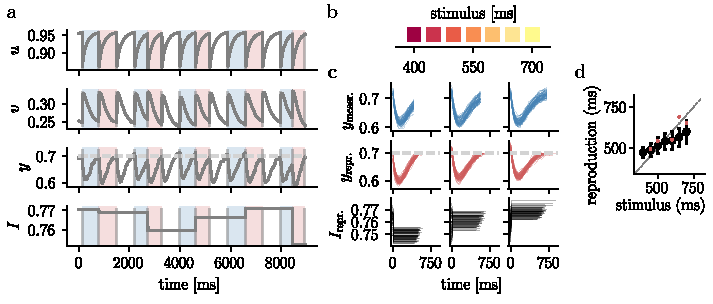
\includegraphics{figures/trial.pdf}
	\caption{\textbf{Simulated reproduction experiment.} 
	\textbf{(a)} The dynamics of $u, v, y $ and $I$ are displayed over time for five consecutive example trials (650, 500, 600, 700, 450 ms) of an experiment simulation with 500 trials. Stimulus presentation and reproduction epochs are highlighted in blue and red, respectively. Before new stimuli presentations, there is a 700 ms delay period (white). Initial values for the experiment simulation are set to $u_0=0.7, v_0=0.2, y_0=0.5, I_0=0.8$. The added noise is set to $\sigma=0.02$ and the memory parameter to $K=5$. The threshold is set to $y_{\text{th}}=0.7$ (dashed line). Reproduced times are 690, 540, 550, 650, 490 ms.
	\textbf{(b)} For the experiment simulation, time intervals were randomly drawn from a discrete, uniform distribution. The range of time intervals contained stimuli from 400 to 700 ms with steps of 50 ms.
	\textbf{(c)} The measurement (upper) and reproduction (middle) epoch of $y$ and input for reproduction (lower) are shown for the full experiment, sorted according to stimulus interval. Shown are trials for stimuli of 400, 550 and 700 ms (depicted above).
	\textbf{(d)} Mean reproduction and standard deviation (black) across trials for each stimulus interval of the experiment stimulation shown (c). If the mean lies on the identity line (dashed line), reproduction time corresponds to the stimulus interval on average. Red dots show the reproductions of the example trials shown in (a). 
	}
\label{fig:experiment}
\end{figure}

Taken together, the model can be applied to simulate realistic time reproduction experiment with many consecutive trials. The noise level and weights were kept throughout the work. 
In contrast to \citeauthor{Egger2020} (\citeyear{Egger2020}), initial values, especially $I_0$ did not need to be adjusted in advance. 
This is because the input will have settled after the first one or two trials and will not be affected by the initial values thereafter.
The mean over the distribution of reproduced time intervals for each stimulus allows for the investigation of the behavioral results (Fig. \ref{fig:experiment}d). 

\section{Model Parameters for Error Minimization}
I asked whether the behavioral effects observed in real data (Fig. \ref{fig:behavioraleffects}) could be reproduced by the circuit model.
For this purpose, I focused on two model parameters, $K$ and $\tau$, and adjusted them to minimize errors in the behavior. 
As mentioned above, other parameters like the noise level and initial conditions were always kept the same. 
The memory parameter $K$ however, is a crucial value to adapt, since it defines the weight with which the input is adjusted to compensate for the discrepancy between the predicted interval and the stimulus duration.
The second parameter that I considered was the time constant $\tau$, which affects how fast the dynamics react in response to the input. Therefore, $\tau$ can be interpreted as a biophysical parameter of the model that describes the rate of a population.
To allow an investigation of the parameters decoupled from the influence of noise, I first used the same stimulus series and second initialized the added noise equally in each simulation. This way, I was able to extract changes in the behavioral results based on parameters only.

For evaluating behavioral characteristics like the range effect, two stimulus ranges were used in simulations, denoted as short and long range. 
The short range contained seven stimuli ranging from 400-700~ms. 
The long range contained the same number of stimuli but was shifted by 300~ms compared to the short range, thus ranging from 700-1000~ms (Supplementary Fig. \ref{sup:CV}a).
 
\subsection{Behaviorally Plausible Time Reproductions}
Before evaluating the behavior of the model, I introduce a more rigorous description of the behavioral effects. 
The regression effect in behavior can be quantified by the slope that results from a linear regression between the stimuli and the reproductions.
Biological plausible slopes lie around 0.83 for the short and 0.73 for the long range (\cite{Sohn2019}, \cite{Henke2021}). 
To evaluate the model, the slopes of behavioral results were obtained for several combinations of the update parameter~$K$ and the time constant~$\tau$.
This resulted in broad parameter regimes in which reproductions show a regression to the mean, as indicated by a slope less than one. 
For fixed $\tau$, the regression increases as $K$ increases, since more weight is given to the current update, and consequently less reliance is placed on the prior. 
The model exhibits biological plausible slopes in the behavior for different time constants (Fig. \ref{fig:parameter}a), where $K$ must be adjusted depending on the stimulus range and time constant. 
To produce plausible slopes, $K$ takes on smaller values for the long range, putting less weight on the update compared to the short range.
This raises the question based on which criteria parameters should be chosen for the simulation.

%Can behavioral effects of magnitude estimation also be achieved by adjusting $K$ and $\tau$ in accordance with error minimization?
\paragraph{Mean squared error to determine model parameters.}
To find suitable parameters independently of the slopes, I minimized the error of mean interval reproductions. The mean squared error (MSE) was defined as $\text{MSE} = \text{bias}^2+\text{var}$, where the bias was expressed as the squared difference between the mean reproduction $\bar{t_{r}}$ for each stimulus interval $t_s$ and variance as mean $\sigma^2$ for all stimulus intervals.
\begin{equation} \label{MSE}
	\begin{split}
	 \text{bias} & = \frac{1}{N} \sum \limits_{i=1}^{N} (\bar{t_{r_i}} - t_{s_i}) \;,\\
	 \text{bias}^2 & = \frac{1}{N} \sum \limits_{i=1}^{N}(\bar{t_{r_i}} - t_{s_i})^2 \;,\\
	 \text{var} & = \frac{1}{N} \sum \limits_{i=1}^{N}(\sigma_i^2) \;.\\
	\end{split}
\end{equation}
This error reflects the trade-off between bias and variance, with the bias error indicating over-assumptions (underfitting) and the variance indicating variability across reproduction and thus sensitivity to noise (overfitting).

\subsection{Model Regime for Error-Minimized Behavior}
Parameters that minimize errors in reproductions, are close to those that result in behaviorally plausible slopes. Furthermore, the effects observed in real data (Fig. \ref{fig:behavioraleffects}) could be reproduced with these parameters.

For increasing time constants~$\tau$, the optimized update parameter~$K$ increases as well. Values of $K$ that minimize errors are smaller for the long range compared to the short range for all $\tau$, as already found for values of $K$ that result in plausible slopes.
The weight parameter that minimizes the MSE for each $\tau$ is denoted as $K^*$. Across time constants,  $K^*$ is slightly lower compared to the weights that yield plausible slopes for the short range. In contrast, for the long range, $K^*$ is slightly larger compared to  weights that yield plausible slopes. Only for very small $\tau$ (below 120~ms), $K^*$ becomes very small.
Although the parameters do not directly coincide, weights that minimize errors are strikingly close to weights that yield plausible behavior (Fig. \ref{fig:parameter}b). 

The time constant that corresponds to the overall minimum of the MSE is denoted as $\tau^*$. 
It differs between the two stimulus ranges:
For the short stimulus range, $\tau^* = 120$~ms and $K^* = 11$ yield an overall minimum, whereas for the long range parameters are $\tau^* = 200$~ms and $K^* = 20$ (For behavioral results cf. Supplementary Fig. \ref{sup:othererror}a, b).
Assuming a constant $\tau$ across experiments, I had to find a shared time constant for both the short and long range. 
Consequently, a time constant between the optima was chosen, considering the overlap with biologically plausible slopes.
With a time constant of 130~ms, optimal $K$ matched with biologically plausible slopes for both ranges (Fig. \ref{fig:parameter}b).
Different noise initialization influence the optimal value of $K$ slightly. For 20 simulations mean $K^*$ and standard deviation for the short range were $K = 12.88$, std = 0.34 and for the long range $K = 8.57$, std = 0.99. 

\paragraph{Behavioral results with error-minimizing parameters.}
Behavioral results of simulations with error-minimizing parameters show a regression to the mean. The range effect is reflected by a stronger regression for the long range (slope of 0.73) compared to the short range (slope of 0.77) (Fig. \ref{fig:parameter}c). 
Furthermore, the standard variation of reproductions increases linearly (scalar variability). The mean coefficient of variation (CV) for the short range is 0.09 and 0.11 for the long range (Fig. \ref{fig:parameter}c).
Summarizing, adjusting $K$ in accordance with error minimization, leads to putting more weight on the prior experience for longer stimuli, which naturally entail more uncertainty, and is thus biologically plausible.
Error-minimized parameter are close to parameters that yield plausible slopes and key behavioral effects are reproduced.
However, for all optimized values, there is a general underestimation of stimulus intervals for the long range, which becomes appeared in Supplementary Fig. \ref{sup:othererror}e.
For dynamics of $y$ for single trials over the course of the experiment, see Supplementary Fig. \ref{sup:experiment}.

\paragraph{Parameters choice based on minimal bias and variance.}
Next, I disentangled the MSE and investigated the contributions of variance and (squared) bias separately (Eq. \ref{MSE}).
If error-minimization is based on the squared bias, $\tau^*$ is smaller for both stimulus ranges. This means, the variance is pushing the optimal time constant to lager values. %100 ms for the short and 110 ms for the long range. 
Similarly, $K^*$ is pushed to lower values by the variance (Supplementary Fig. \ref{sup:othererror}c, d).
No range effect can be observed when minimizing the error in reproductions based on the squared bias or the variance. 
Moreover, relation of stronger weighting of the prior for the long range due to decreased $K$ is not apparent for either error metrics (Supplementary Fig. \ref{sup:othererror}c, d).
This is why I conclude, that the MSE is a suitable choice to determine $K$ and $\tau$.


\begin{figure}[ht]
	\centering
	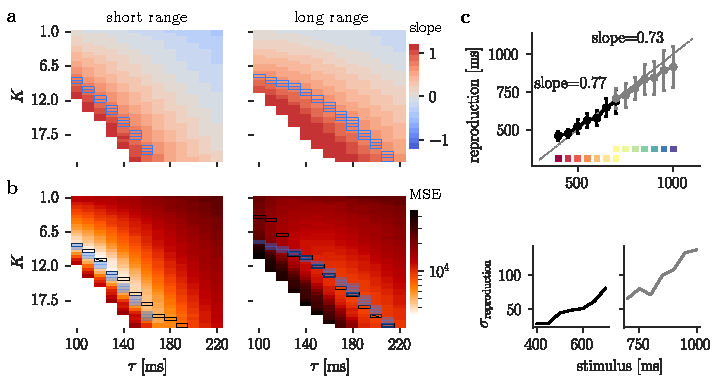
\includegraphics{figures/interIparams.pdf}
	\caption{\textbf{Time reproductions with parameter that minimize errors.} 
	\textbf{(a)} Simulations with 500 trials for each pair of memory parameter $K$ and time constant $\tau$ at noise level $\sigma = 0.02$. Simulations were performed with stimuli chosen from the short (left) or long range (right). Color scale represents the slope of the linear fit between stimuli and reproductions. A slope of 1 on the identity line corresponds to perfect reproduction of the stimuli. Behaviorally plausible slopes are encircled in blue and lie around 0.83 for the short and 0.73 for the long range. Empty space corresponds to simulations, that exceeded the number of timeout trials and were thus excluded from analysis.
	\textbf{(b)} Optimization of the weight given to the update $K$ for different time constants $\tau$ at noise level $\sigma = 0.02$. Color scale represents the MSE for an experiment stimulation with 500 trials for each pair of $K$ and $\tau$. Stimuli were either chosen from the short (left) or the long stimulus range. The minimal error for each $\tau$ is encircled in black and minimal error across all $\tau$ is additionally crossed. Parameter combinations that result in behaviorally plausible slopes (a) are shaded in blue.
	\textbf{(c)} Top: Mean reproductions for simulation with 500 trials for each stimulation with the short (black) and long (gray) stimulus range. The value of $K$ is optimized for a time constant of $\tau = 130$ ms. For the simulation with short stimulus range $K^*$ was 13, with the long stimulus range optimal $K^*$ was 10. 
		The slope is the result of a linear regression between stimuli and reproductions.
		Inset: For experiment simulations two stimuli ranges were used. The short range contained stimuli from 400 to 700 ms, the long range contained stimuli from 700 to 1000 ms.
		Bottom: Standard deviation of reproductions for each stimulus for the short and long range from the simulation in (c).
	}
\label{fig:parameter}
\end{figure}

\subsection{High Input Regime}
Even tough, there are differences between the intermediate and high input regime in terms of fixed points and dynamics, simulations of time reproduction experiments are possible in both regimes. 
One reason to look closer at the high input regime is, that the dynamics of $y$ all converge towards the same steady state, whereas in the intermediate input regime, for different inputs, $y$ evolves towards different steady states. 
In the following, I investigate simulations in the high input regime and compare results with those in the intermediate input regime.

\paragraph{Comparison of dynamics to the intermediate input regime.}
While in the intermediate input regime three fixed points emerge in the phase plane (two stable and one unstable), in the high input regime the fixed points merge to a single one. 
The single fixed point is located at comparatively high activity of $u$ and $v$ 
(Fig. \ref{regimes}b, d).
This affects the dynamics of $u$ and $v$ such that $y$ ramps up in instead of down as observed in the intermediate regime. 
Increasing $I$ results in steeper activity of $y$ in the high input regime. This is reversed compared to the intermediate input regime, where an increased $I$ leads to flatter slopes in $Y$ (Fig. \ref{regimes}a, c). 

\begin{figure}[ht]
	\centering
	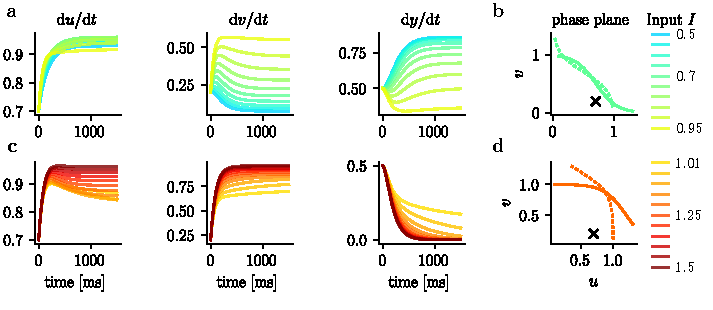
\includegraphics{figures/supp_regimes.pdf}
	\caption{\textbf{Comparison of dynamics in the intermediate and high input regimes.} 
	\textbf{(a)} Evolution of $u, v$ and $y$ over time for different inputs from 0.5 to 0.95 in the intermediate input regime. Activity in $y$ shows a ramping-up activity. The activity of $y$ evolves to different steady states depending on the input. 
	\textbf{(b)}  The phase plane in the intermediate input regime shows two stable and one unstable fixed point. The nullclines of u (dashed) and v (solid) are shifted to higher activities when the input I is increased. The plot shows nullclines corresponding to an input of 0.7 and the black marker indicates the initial condition of dynamics in (a).
	\textbf{(c)} Same as (a) for the high input regime with inputs from 1.01 to 1.5. Activity in $y$ shows a ramping-down activity, converging to 0 independent of input.
	\textbf{(d)} Same as (b) for high input regime.  The phase plane in the high input
	regime shows one stable fixed point. The nullclines of u (dashed) and v (solid) are
	shifted to lower activities when the input $I$ is increased. The plot shows nullclines corresponding to an input of 1.2 and the black marker indicates the initial condition of dynamics in (c).
	}
\label{regimes}
\end{figure}

\paragraph{Experiment simulation and error-minimizing parameters.}
To simulate time reproduction experiments in the high input regime, the following changes must be made. 
The threshold was set to a value lower than 0 (e.g. 0.1) and initial $I$ was increased to a value above 1 ($I_0 = 1.02$). The reset impulse after each epoch had to be stronger by a factor of 10 and with opposite sign to bring the activity in $y$ back to a higher level.

\begin{equation} \label{EqhighI}
	\begin{split}
	\tau\frac{\text{d}u}{\text{d}t} & = -u + \theta(W_{uI}I - W_{uv}v + \eta_u + 10*I_r) \;,\\
	\tau\frac{\text{d}v}{\text{d}t} & = -v + \theta(W_{vI}I - W_{vu}v + \eta_v - 10*I_r) \;.\\
	\end{split}
\end{equation}

There is no need to change the update mechanism, even though the relation of the input $I$ and the slope is reversed. This is because $y$ approaches the threshold from above and not from below, so the relation of $y$ and $y_{\text{th}}$ is reversed and the update of $I$ is correct. 

The noise was set to the same value as in simulations in the intermediate regime ($\sigma$ = 0.02). The standard deviations increased linearly. For increasing $\sigma$ the standard deviation drops slightly and then plateaus for $\sigma$ larger than 0.1. The CV has similar values as in the intermediate regime with 0.13 for the short and 0.12 for the long range for a $\sigma$ of 0.02 (Supplementary Fig. \ref{sup:highI}a). 
An example of the experiment dynamics for four consecutive simuli is displayed in Fig. \ref{highI}a.

%\paragraph{Error-minimizing parameters }
Just as for the intermediate input regime, I identified parameters $K^*$ and $\tau^*$ that minimize the MSE of reproductions. 
Again, the model is able to produce biologically plausible slopes for most time constants (Supplementary Fig. \ref{sup:highI}b). The weight $K$ that minimized errors is smaller compared to the weights that yield plausible slopes for both ranges. 
For all $\tau$ larger 40~ms, optimal $K$ is smaller for the long range compared to the short range (Supplementary Fig. \ref{sup:highI}c).
The MSE is minimal for $\tau^* = 60$~ms for both the short and the long range, with $K^* = 4$ and $K^* = 2.5$  for the short and the long range, respectively. 
Behavioral results of experiment simulation with error-minimizing parameters show a regression to the mean.
For the long range the regression has a slope of 0.68 and for the short range the slope is 0.74, hence a range effect is present.
In contrast to the intermediate input regime, however, standard deviations of the reproductions do not grow linearly in the long range (Fig. \ref{highI}b).
For dynamics of $y$ over the whole experiment see Supplementary Fig. \ref{sup:experiment_high}.

\begin{figure}[ht]
	\centering
	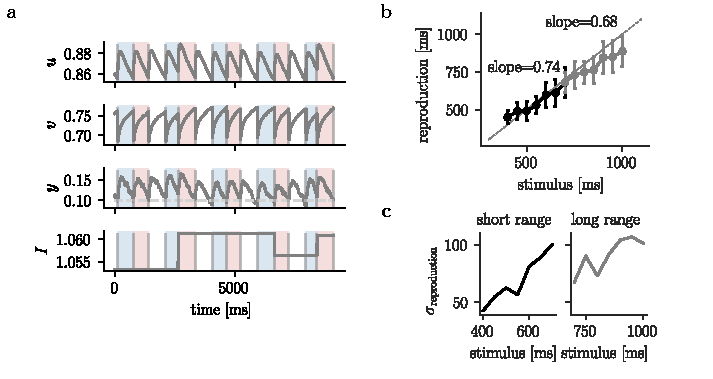
\includegraphics{figures/highI.pdf}
	\caption{\textbf{Experiment simulation in the high input regime.} 
	\textbf{(a)} Activity of $u, v, y$ and $I$ for five example stimulus intervals of 650, 500, 600, 700, 450 ms. Stimulus presentation and reproduction epochs are highlighted in blue and red, respectively. The delay period between trials is shown in white. Initial values are set to $u_0=0.8 , v_0=0.6 , y_0=0.1, I_0=1.04$ and the threshold $y_{\text{th}}$ is set to 0.1. 
	\textbf{(b)} Top: Mean reproductions for simulation with 500 trials for each stimulation with the short (black) and long (gray) stimulus range. The value of $K$ is optimized to minimize errors in reproductions for a time constant of $\tau = 60$ ms. For the simulation with short stimulus range optimal $K$ was 4, with the long stimulus range optimal $K$ was 2.5.
		The slope is the result of a linear regression between stimuli and reproductions.
		Bottom: Standard deviation of reproductions for each stimulus for the short and long range from the simulation in (b).
	}
\label{highI}
\end{figure}

\paragraph{The high input regime provides no improvement of.}
The common steady state in the high input regime was an intriguing feature.
However, previous results have shown that the intermediate regime exhibits behavior closer to characteristic effects found in time estimation, e.g. monotonic increase of standard deviations of the reproductions. 
To compare one last property, I looked at the relation of the mean input in the reproduction epoch for each stimulus in an experiment.
The mean input $I$ an almost linear increase (or decrease for the high input regime) within a range. The increase (or decrease) is shallower for the long range due to the lower $K^*$ used in the simulation (Fig. \ref{fig:comparison}b, d).
The maximum and minimum input $I$ during the simulation for the short or the long range were used to examine the most distant nullclines of $u$ and $v$ in the phase plane(Fig. \ref{fig:comparison}a, c). 
In the intermediate regime, the difference between maximal and minimal $I$ is larger and the nullclines are also further apart. Other than that, no difference can be identified between the regimes. 
Taken together, the high input regime offers no improvement, if not a deterioration over the intermediate regime. Therefore, I discarded the high input regime and based the following analysis only on the intermediate regime. 

\begin{figure}[!htb]
	\centering
	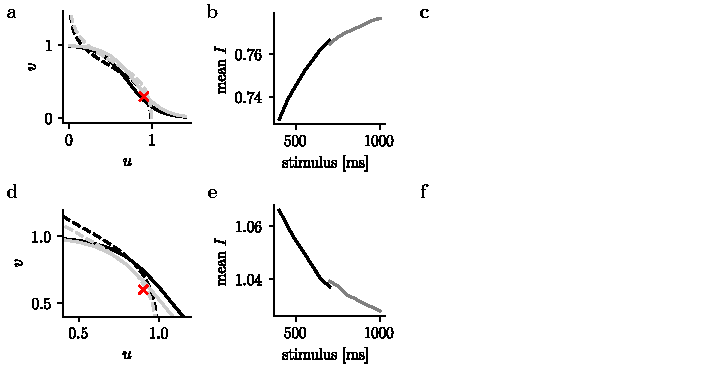
\includegraphics{figures/supp_comparison.pdf}
	\caption{\textbf{Comparison of experiment simulations.}
	\textbf{(a)} The phase plane in the intermediate input regime shows two stable (blue) and one unstable (light blue) fixed point. The nullclines of $u$ (dashed) and $v$ (solid) are displayed. Black and gray nullclines correspond to an input of 0.71 and 0.79, respectively, which corresponds to the maximal and minimal input in the experiment simulation for the short and long range in Fig. \ref{fig:parameter}c.
	\textbf{(b)} Mean input during the reproduction epoch for each stimulus of the short (black) and long (gray) range for the experiment simulation in the intermediate input regime with optimized parameters from Fig. \ref{fig:parameter}c.
	\textbf{(c)} The phase plane in the high input regime shows one stable (blue) fixed point. The nullclines of $u$ (dashed) and $v$ (solid) are displayed. Black and gray nullclines correspond to an input of 1.081 and 1.017, respectively, which corresponds to the maximal in minimal input in the experiment simulation for both the short and long range in Fig. \ref{highI}b.
	\textbf{(d)} Same as (b) for the experiment simulation in the high input regime with optimized parameters from Fig. \ref{highI}b.
	}
\label{fig:comparison}
\end{figure}

\section{General Underestimation of Reproductions}
The indifference point of the reproductions to the stimuli is shifted to lower values in the long range.
However, because of the central tendency of reproductions, the indifference point of a linear regression between stimuli and reproductions should correspond to the mean of the stimulus range.
This is the case for the short range, where the indifference point corresponds to 595~ms, which is close to the range's mean value of 550~ms. For the long range, the indifference point is 710~ms, and thus considerably smaller than the range's mean of 850~ms (for behavioral results cf. Fig. \ref{fig:parameter}c). This means that simuli in the long range are in general underestimated. 

What is the reason for the general underestimation of larger inputs? 
It is not uncommon for stimuli in larger ranges to be generally underestimated in magnitude estimation across time domains. Time reproduction experiments with gerbils show a general underestimation across ranges (Fig. \ref{fig:underestimation}a, \cite{Henke2022}). 
The cause has not yet been researched and could be due to many reasons ranging from lapsing attention to impatience. 
It is necessary to investigate whether the underestimation in the model's behavioral output is caused by the regime in which the model operates, or whether it is a phenomenon that arises from optimal choice of parameters.
Possible parameters of the model that could influence the behavior are the delay period between trials, the fixed threshold and the common time constant between stimulus ranges.

\subsection{Time Constant and Delay Period Influence Reproductions}
Adjusting the time constant can counteract the general underestimation of reproductions.
Simulations in the previous sections were performed with a common time constant $\tau$ that was set between the optimal $\tau^*$ for the short and long range, respectively.
General underestimation in simulations with the long range can be compensated by increasing the time constant towards the optimum of the long range. However, this causes a general overestimation in the simulation with the short range (Supplementary Fig. \ref{sup:othererror}b). 
Thus, a common time constant $\tau$ contributes to the under- and overestimation of stimuli, when it's too far from the optimum of the range. However, even with optimal $\tau$, simulations show a slight general underestimation in the long range.
Hence, there had to be several causes for this problem.

\paragraph{The delay between trials causes skewed reproductions.}
For both the long and short range, the best reproductions were obtained for stimuli near 700~ms.
Following this observation, I simulated an experiment with a stimulus range that was situated around 700~ms, ranging from 550 to 850 ms. 
The mean of 700~ms corresponds to the maximum of the short range and the minimum of the long range, and also complies with the length of the fixed delay period between trials.
In Fig. \ref{fig:delay}a the behavioral results show regression to the mean with a slope of 0.82 and an indifference point of 657~ms.
When setting the delay period at the maximum of the long range instead (1000 ms), a general overestimation of stimuli from the short range occurs (Supplementary Fig. \ref{sup:delay}c).
This led to the assumption that a delay period too far from the range's mean leads to under- or overestimation. 
A comparatively short delay period compared to the mean of stimuli leads to distorted updates, because $y$ cannot reach the threshold in the short time period with mean input strength $I$. 
After resetting, the following measurement period is started from lower values in $y$. 
Setting the delay period equal to the mean of the short or long range 
eradicates general underestimation (Supplementary Fig. \ref{sup:delay}a, b).

\subsection{Adjusted Experiment Simulation}
The previous analysis showed, that there are two main problems that caused distorted stimulus reproductions. 
First, a common time constant between experiments with different ranges skews the reproductions.
Second, the experimental design should not bias reproductions, however the choice of the delay between trials interferes with correct reproductions. %The delay period between trials should not influence reproductions.

Since the time constant in the model can be interpreted as a rate time constant, it is justifiable to adapt it between experiment with different stimulus ranges. 
This would correspond to a firing rate adjustment in the population to an experimental setting.
In a biological system, an inhibitory population could scale the rate time constant according to the stimulus statistics.
%todo: K not comparable across ranges (not smaller for long range etc)

\paragraph{The delay period is omitted in the experimental design.}
Furthermore, the model needs to be adjusted to take into account the impact of the delay period on the reproductions. 
% delay=mean of range
Setting the delay time to the mean of the stimulus range used in the simulation doesn't make sense from a design perspective. It should be possible to choose the delay period between trials arbitrarily and independently of the stimulus range. 
% long delay + separate tau
Similarly, the delay period could be chosen long enough to allow the system to evolve to a steady state. However, this would mean that the delay time cannot be chosen independently.
% no delay

Another way to solve the problem of the delay epoch, is to neglect the delay in the simulation of the experiment (Fig. \ref{fig:delay}b).
The reproduction period always ends when the threshold $y_\text{th}$ is met. If the measurement period of the subsequent trial follows directly after it, it always starts at the same value of $y$. 
This does not necessarily mean, that the experimental design is limited. When simulating experiments that include a delay period between trials or even between measurement and reproduction epoch, it can be assumed that information is stored in the system until the beginning of the next epoch. 
In neural networks, it has been shown that the timing information in the state space can be held over a delay time (\cite{Bi2020}).
Neglecting the delay epoch in combination with independent $\tau^*$ for each range leads to characteristic effect and biologically plausible slopes (Fig. \ref{fig:delay}c).
% reset on fixed value
% learn I for delay
Solutions that incorporate a delay period into the simulation itself would require model adjustments.
Either the reset is changed from an impulse to a fixed reset value, or the input is updated separately during the delay epoch based on an error to always reach the threshold. 

Unless otherwise specified, error-minimizing $\tau^*$ and a delay of 0~ms are used for each stimulus range in following simulations. The regime of $I$ remains similar to previous simulations with delay and common $\tau$. There is an overlap in $I$ and $K$ is no longer comparable due to separate $\tau$ between different ranges (Fig. \ref{fig:new_ranges}b).

\begin{figure}[ht]
	\centering
	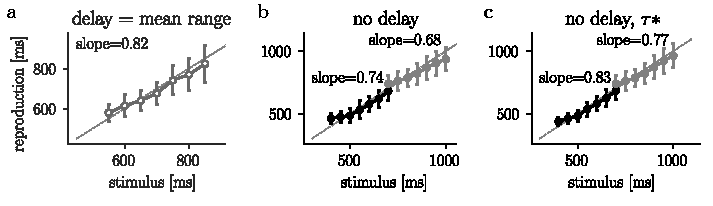
\includegraphics{figures/delay.pdf}
	\caption{\textbf{Behavioral results with altered delay.} 
	\textbf{(a)} Behavioral results of an experiment simulation with the previously utilized delay of 700 ms. The stimulus range that was used to sample stimuli from has a mean equal to the delay of 700 ms. The time constant and update parameter were both optimized based on the MSE ($\tau$ = 170 ms, $K$ = 17.5). Other parameters like threshold and initial values were not changed. 
	\textbf{(b)} The delay period was set to 0 ms in simulations with the short and long range (black and gray, respectively). The time constant was set to 165 ms, which corresponds to the mean of the optimal $\tau$ for the short (130 ms) and long (200 ms) range. For $\tau$ = 165 ms, the update parameter $K$ was optimized (short range $K$ = 21, long range $K$ = 13). Note different axes of figures in (a) and (b).
	\textbf{(c)} Same as (b) but with independent, optimal time constant. For the short range $\tau^*$ = 130, $K$ = 14 and for the long range $\tau^*$ = 200, $K$ = 20.
	}
\label{fig:delay}
\end{figure}

\section{Influence of External Variability on Behavior} \label{externalvar}
Time reproductions are affected by internal noise and external variability of stimuli.
Performance in time reproduction depends on the discrimination abilities of the individual subject. In the model, this is reflected by internal noise $\sigma$.
But time reproductions not only depend on the current stimulus interval, but also on context information and task-irrelevant influences (\cite{Bausenhart2016}).
Variability of the environment is captured by the statistics of stimuli over the course of an experiment. 
When internal noise is fixed, the external variability can be modified independently. 
In this section, I examine the effects of external variability on the behavior of the model, by changing the mean and the variance of stimuli separately. 
By comparing the behavioral results of the model with data from gerbils and humans, I find similarities and discrepancies that raise unresolved questions.

\paragraph{Effects of stimulus statistics in real behavior}
With larger time intervals, internal estimates get noisier and regression of reproductions gets stronger. This is well described by the \textit{range effect} across species (\cite{Cicchini2012}, \cite{Sohn2019}), \cite{Henke2021}, \cite{Henke2022}. 
Besides the mean, also the variance of stimuli could influence the reproduction.
Larger variance can be achieved by reducing the sampling frequency of the stimulus range or by expanding the width of the range, accommodating more distant time intervals. 
The effect of changing the variance of stimuli on the behavior has not been well studied.
There are three different effects that greater variance could have on behavior. 
Reproductions could improve, leading to a weaker regression. This would mean that subjects rely less on the prior. 
Intuitively, larger variance means that differences of time intervals get more apparent and discrimination becomes easier (e.g. stimuli are further apart or extremes are more distinct). 
This scenario is predicted by a model that uses noisy integrators linked by an adaptive reference in \citeauthor{Thurley2016} (\citeyear{Thurley2016}).

On the other hand, a change in variance might have no effect on behavior, if the mean is fixed. According to this, only the mean value would have an influence on the reproduction performance.
This seems to be the case in \citeauthor{Petzschner2012} (\citeyear{Petzschner2012}), since performance of the range with larger variance doesn't get better. 
Finally, reproductions may be worse with greater variance. This was demonstrated in the case of sound intensity estimations by \citeauthor{Teghtsoonian78} (\citeyear{Teghtsoonian78}).
In most studies that included experimental data with varying variance of stimuli, the effects on regression were not examined. 

\subsection{Optimality Predicts Key Effects}
To test the behavior of the model with respect to the external variability of stimuli, additional ranges were introduced, differing in mean, width, and sampling frequency.
The short and the long range include seven stimuli spanning 300 ms, with mean values of 550 and 850~ms, respectively. 
Two ranges had the same variance and width, but shifted mean values at 700~ms (mid range) and 1050~ms (extra-long range). With increasing mean, the range effect predicts a flatter slope. 
In addition, ranges were examined whose mean was equal to one of the ranges above, but which had a higher variance.
Including all stimuli from the short and the long range, the all range has the same mean as the mid range, but a larger width (600 ms) and therefore higher variance.
The short-few and all-few range encompasses the short and the all range, respectively, but with smaller number of stimuli, the variance increases in both cases 
(Fig. \ref{fig:new_ranges}a, Supplementary Fig. \ref{sup:ranges}c).
%%%%%%%%%%%%%%%%%%%%%%%%
%Optimal $\tau^*$ for stimulus ranges are as follows: short~130~ms, mid~170~ms, long~200~ms, extra-long~230~ms, all~150~ms, ~short-few~120~ms and all-few~160~ms.

For all ranges, the slope of the linear regression between stimuli and reproductions is below one. Thus, simulations with error-minimizing parameters predict the regression effect across several ranges. 
The slopes decrease significantly as the mean of the stimulus range increases, except for the short and mid range (Fig. \ref{fig:new_ranges}c).
Thus, the model predicts the range effect only for sufficiently large changes in the mean. 
(Kolmogorov-Smirnov two-sample test, p$<$0.01, n=21 for each distribution, Bonferroni correction for multiple testing).
Across ranges that only change their mean value (short, mid, long and extralong), the slope has a linear correlation with the mean value of the range (Pearson correlation r=-0.95, $p<0.05$).

When the experiment was simulated with a common $\tau$ of 165~ms between ranges, $K^*$ is significantly lower for the mid range (16.71) compared to the short range (21.33), but slopes show no significant difference (Supplementary Fig. \ref{sup:ranges}a, b).
Decreasing $K^*$ for increasing mean of ranges is captured by the model beyond the short and the long range.
(Kolmogorov-Smirnov two-sample test, n=20 for each distribution, p$<$0.01, Bonferroni correction for multiple testing).\\

%%%%%%%%%%%%%%%%%%%%%%%%%Grenzen des Models%%%%%%%%%%%%%%%%%%%%%%%%%%%%%%%
%underestimation extra long: grenzen des Models, breaks down
%reason for range effect
\paragraph{What causes the range effect in the circuit model?} 
The model is situated in a dynamic regime, that displays time reproductions close to real behavior.
Error-minimizing parameters predict the regression and range effect across multiple stimulus ranges.
Decreasing slopes for larger stimulus ranges occur because they approach the limit of the dynamic regime (Fig. \ref{fig:new_ranges}b).
When the stimulus ranges are pushed to more extreme values, the behavior of the model breaks down. Reasons for a breakdown are large numbers of timeouts in the case of too short time intervals. If time intervals are too long, the variance in reproductions increases sharply and $K$ is pushed to lower values, resulting in slopes that are well outside the observed behavior. 
This means that the regime of the model has to be adapted to major changes in the external statistics. 

\subsection{Optimality Predicts no Effect of Variance on Behavior}
How does the slope change when the mean of stimuli remains constant, but variance is increased?
The statistics of stimuli can be summarized by the ratio of the mean and variance of the stimulus range: $\frac{\text{E(t)}}{\text{Var(t)}}$.
Higher variance in ranges with lower stimulus sampling (short-few, all-few) shows no significant difference from their counterparts with normal stimulus sampling (short, all).
Furthermore, a larger width of stimuli does not result in a significant larger or smaller slope (all range vs mid range).
Therefore, increasing variance is not affecting the reproduction of stimuli in the model (Kolmogorov-Smirnov two-sample test, n=21 for each distribution, Bonferroni correction for multiple testing).
Considering only the mean, there is a significant correlation with the slope (Pearson correlation r=-0.96, $p<0.001$), but not with the external variability ratio (Pearson correlation r=-0.65, $p=0.12$) (Fig. \ref{fig:new_ranges}c).
In the simulation with a common $\tau$ there is no significant difference in $K^*$ when the variance is changed (Supplementary Fig. \ref{sup:ranges}a, b).
However, increasing the variance of a range leads to a significant increase in MSE in all cases (Fig. \ref{fig:new_ranges}d).  
(Kolmogorov-Smirnov two-sample test, n=21 for each distribution, p$<$0.01, Bonferroni correction for multiple testing).

\begin{figure}[ht]
	\centering
	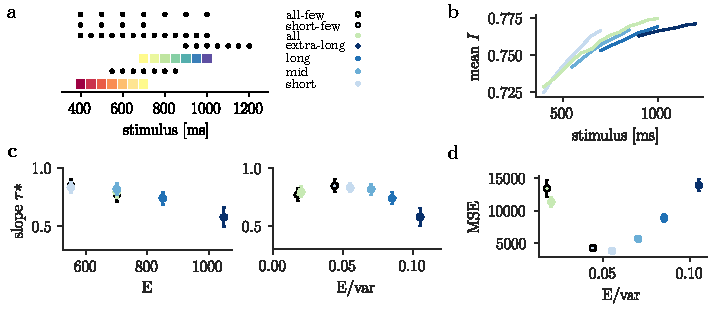
\includegraphics{figures/ranges_new2.pdf}
	\caption{\textbf{Behavioral slopes with varying stimulus statistics.} 
	\textbf{(a)} Parameter simulations were performed with stimulus ranges that differed in mean and variance to the short and long range. The mid range has its mean at the overlap of the short and long range. The extra-long range has its mean above the long range. Both the mid and extra-long range contain seven stimuli, just as the long and short range. To change the variance a range with 13 stimuli that span the short and long range was included (all range). Both the short and the all range were for the short-few and all-few range under sampled.
	\textbf{(b)} Simulations were performed with optimized $\tau^*$ (and corresponding  $K^*$): short 130 ms (14), mid 170 ms (17), long 200 ms (20), extra-long 230 ms (18), all 150 ms (14). Mean input $I$ for each stimulus was calculated for stimulation with different ranges. Colors correspond to legend in (a). 
	%short-few 120 ms (12) and all-few 160 ms (15)
	\textbf{(c)} Left: Slopes of behavioral results plotted against the mean of the range that was used. The error bars indicate standard deviation in the slope for different initialization. Colors correspond to legend in (a).
	Right: Slopes plotted against the ratio of the mean and the variance of each range. 
	\textbf{(d)} The MSE for simulations with error-minimizing parameters plotted against the ratio of mean and variance of the range.
	}
\label{fig:new_ranges}
\end{figure}

\subsection{Comparison of Model Output to Real Data}
The circuit model predicts that a change in variance affects the MSE \todo{use glossary} of the reproductions.
It also predicts, that only the mean and not the variance has an effect on the regression of reproductions, which is in contrast to the noisy integrator model proposed by \citeauthor{Thurley2016} (\citeyear{Thurley2016}).
In the following section, I compare predictions of the model with behavioral data from time reproduction experiments with gerbils and humans. The stimuli in these experiments were several seconds long and came from either a short, mid, long or all range (data by Henke and Thurley).
\todo{cite here the data, link or paper}

Behavior in gerbils exhibits a regression effect for all ranges and a range effect for ranges with increasing mean. 
The variation in slopes between gerbils is considerably larger when the variance is increased.
At the individual level, both consistent and increasing performance with increasing variance is observed. 
There are three gerbils that show a linear increase in performance with decreasing ratio of the mean and variance of the stimulus range (Fig. \ref{fig:underestimation}b). The remaining four gerbils however, show no effect of variance on reproductions (Supplementary Fig. \ref{sup:underestimation}a).
On average Pearson correlation shows a significant linear relation of the slope with the mean (r=-0.62, $p<0.001$) and ratio of mean and variance (r=-0.61, $p<0.001$) in gerbils.
This correlation gets stronger when the all range is excluded (r=-0.75, $p<0.001$).
In humans, behavior is heterogeneous, and there is no range effect on average, but there is in some individuals (Fig. \ref{fig:underestimation}). There is no significant correlations of the slope with the mean or external variability ratio.
The root MSE increases as the variance increases across all subjects (Supplementary Fig. \ref{sup:underestimation}b).

%%%%%%%%%%%%%%%%%%%%%%%%%% comparison
The circuit model predicted no effect of variance on the regression, but on the error in reproductions. 
Gerbils show a discrepancy in performance when variance is increased. 
The model captures only one possible behavior, namely not taking into account a change in variance. 
There is no significant correlation of the slope with the external variability ratio in the model, when in gerbils there is.
\todo{Check what you mean by this}
However, the model predicts correctly increasing error in reproductions with higher variance (Fig. \ref{fig:new_ranges}b).


%EVAR all:    g r=-0.61, $p<0.001$, h r=-0.05, $p=0.802$, m r=-0.64 $p=0.12$
%E all:       g r=-0.62, $p<0.001$, h r=-0.08, $p=0.718$, m r=-0.96, $p<0.001$
%EVAR(E) sml: g r=-0.75, $p<0.001$, h r=-0.4, ???       , m r=-0.95, $p<0.05$

\begin{figure}[ht]
	\centering
	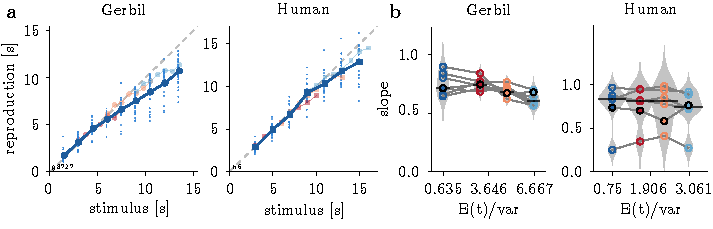
\includegraphics{figures/underestimation.pdf}
	\caption{\textbf{Effects of stimuli statistics on behavior of gerbils and humans.}
	\textbf{(a)} Representative behavioral results of time reproduction of a gerbil (left) and a human (right). Stimuli were several seconds long. Four experiments were conducted with different ranges: short (red), mid (orange), long (light blue) and all (blue). Large markers display the mean of trials. Small dots show reproductions of single trials for the experiment with the all range.
	Ranges differed slightly between experiments with gerbils and humans. 
	\textbf{(b)} Slope of the linear regression between stimuli and reproductions for seven gerbils (left) and six humans (right) plotted against the ratio of the mean and variance of the stimulus ranges. Vertical black markers indicate the median of slopes and gray violin plots illustrate the distribution over all animals. Slopes for different stimulus ranges of one animal are connected by lines. 
	Figure courtesy of Kay Thurley and Josephine Henke.
	}
\label{fig:underestimation}
\end{figure}

%%%%%%%%%%%%%%%%%%%%%%%%%%%%%%%%%%%%%%%%%%

\section{Discussion}
Previous results indicated, that time is encoded in dynamical changes of population activity, the rate of which is adjusted to the expected timing of movement initiation (\cite{Remington2018}, \cite{Wang2018}, \cite{Egger2019}, \cite{Henke2021}).
This led to the hypothesis, that control over timed behavior can be understood in terms of adjustments to initial conditions and external inputs of a dynamical system (\cite{Tsao2022}, \cite{Remington2018}, \cite{Wang2018}).
Further support was provided by the study of RNNs, that were trained on time reproduction tasks. When trained with a tonic input, RNNs generated smooth temporal scaling when exposed to novel inputs. This was not the case for RNNs trained on transient inputs, supporting the hypothesis of the speed-control mechanism via a tonic input (\cite{Remington2018}, \cite{Bi2020}, \cite{Zhou2022}).
The circuit model takes the core of this mechanism i.e. a dynamical systems approach and combines it with other evidence, like an action triggering state or an error signal, to facilitate time reproduction. 

Speed control is implemented via a tonic input to two neurons, such that the readout unit scales its activity with the input and reaches a fixed threshold at different times, corresponding to the triggering of a response.  
The threshold corresponds to the action-triggering state in the population activity, when the neural trajectory is projected onto the time axis (\cite{Remington2018}).
In each trial, the model updates the input according to the stimulus interval.
Previous work showed that the population dynamics are sequentially updated based on an error signal to yield better estimates (\cite{Egger2019}).
In the model, the error signal is extracted in the measurement epoch from the distance of the read-out activity to the threshold. The error is combined with a weight and used to either increase or decrease the input to match the time of threshold crossing to the stimulus interval in the reproduction.
For judgments about time, the brain is thought to rely on an internal reference, that is sequentially updated over trials (\cite{Dyjas2012}, \cite{Bausenhart2014}). This concept is tightly connected to a Bayesian framework of magnitude estimation, where a prior is combined with current estimates (\cite{Shi2013}, \cite{Petzschner2015}).
In the circuit model, the input level in the measurement is inherited from the previous trial and updated before the reproduction epoch based on the weighted error.
Thus, the inherited input to the measurement epoch is composed of the initial input and all past updates, which can be interpreted as a moving average of preceding inputs. 
The mean input over the course of an entire experiment reflects the prior or internal reference in the circuit model, corresponding to the mean stimulus interval. 
\todo{ausbauen und motivieren, bessere darstellung der daten wang 2018}
To better approximate the prior or internal reference hypothesis, the input in each measurement epoch could be set to a value equal to the moving average of the previous inputs, rather than being inherited from the previous trial.  
Taken together, the model uses the core elements that have been observed in data, but in a simplified way, making it possible to study the resulting dynamics in depth. 
It has already been shown that the model captures the classical effects of magnitude estimation when fitted to human data (\cite{Egger2020}).

%-----> summary what shown
%what is the prediction of the model? what does the data say? 
Here, I extended the model to simulations of realistic time reproduction experiments that reflect stimulus variability by presenting random time intervals drawn from a stimulus distribution.

\subsection{Representation of Stimulus Statistics}
Simulations across a variety of stimulus ranges confirmed, that the model captures classical behavioral effects in realistic experiment settings under a parameter regime that minimizes errors in reproductions. %such as the regression effect, the range effect and scalar variability
This suggests, that adjusting neural dynamics based on an internal reference in the presence of noise could lead to the key effects found in time reproduction experiments such as the regression effect, the range effect and scalar variability. 
\citeauthor{Sohn2019} (\citeyear{Sohn2019}) suggested that optimal integration of prior beliefs arise from the curved nature of neural trajectories. Based on the results from the circuit model, curvature of manifolds would not be necessary to achieve biases in the reproduction, as they result from a sequential weighted update of the speed command (external input), where the weight is adjusted based on the stimulus statistics. 

Since the key effects of time estimation were reproduced in simulations, I tested additional parameters in the stimulus statistics, e.g. modifying the variance of the stimulus distribution, to test the model's behavior for different external variability.
Only few studies have investigated an internal representation of temporal statistics. \citeauthor{Acerbi2012} (\citeyear{Acerbi2012}) showed that humans are able to represent the statistics of stimulus distributions to their third moment in reproductions.  
However, the model did not predict an impact of the change in external variability on the regression effect, but did predict an impact on the error in reproductions.
This finding was partially confirmed in gerbil data, but some animals differed from the group by accounting for the change in variance, as evidenced by an increase in performance of interval reproductions.
Animals that considered the variance in the data seem to have adapted to the new stimulus statistics in contrast to the other animals. 
How neural dynamics adjusted to accommodate the new information provided by changed variance is still to be determined.
\citeauthor{Meirhaeghe2021} (\citeyear{Meirhaeghe2021}) examined the adaptation to simultaneous changes in variance and mean of stimuli and identified modulations in the firing rates and adjusted speed in the population dynamic to take into account the new distribution mean. The influence of variance, however, was not investigated separately. 
Understanding how external stimulus statistics feed into the computations of timing in the brain can help us better understand the underlying mechanism. 
Further experiments should be conducted to investigate this shift to considering information from altered stimulus statistic. 
By gradually changing the variance the difference between animals in when and if adaptation occurs, could be revealed. \todo{check language}
Animals that did not increase performance in the present data might do so, if the variance is further increased.
Based on new evidence, the model would need to be extended to account for this adaptation in dynamics that improves performance.
%Solution: Discuss initial conditions that set state play role in \cite{Remington2018}
% Finally, for temporal expectation, the learned period of expectation is reflected through a shift in popu­lation state that reflects the predictable external temporal structure

\subsection{Scales of Timing}
% msec perceptual timing, sec time estimation thought to rely on conscious and cognitive control
% there is remapping zwischen ms und s in real data, millisecond to seconds, adaptation due to same effects observed.
Timing encompasses various scales, ranging from milliseconds, seconds to circadian rhythms. This raises the question of how timing mechanisms can accommodate time computations for widely spaced intervals. 
\todo{2 Sätzte was circadian rhythms machen: gene expression cycles (not in second regime), non neural based mechanisms}
While circadian rhythms rely on district mechanisms to encode time, it is not clear whether there are different timing mechanisms between subsecond and suprasecond (\cite{Buonomano2002}, \cite{Buonomano2007}, \cite{Paton2018}, \cite{Tsao2022}). %overlap of mechanims
Neural trajectories encoding time have been identified in both the subsecond (\cite{Sohn2019}, \cite{Meirhaeghe2021}) and suprasecond scale (\cite{Henke2021}), though adaptations of dynamics seem to take place.
This becomes apparent when comparing the regression effect between experiments conducted with ranges in different timescales. 
The range effect does not propagate from the subsecond scale to ranges in the suprasecond scale, in other words, the slopes for regression are independent and start close to 1 for short ranges in the suprasecond scale. 

Simulations with the circuit model revealed that there is a limited regime in which the model exhibits the classical magnitude estimation effects. 
For stimulus ranges that are much larger or smaller than those I used, the behavior of the model breaks down.
This means that when the model is used in experiments with even shorter or longer time intervals, the operating regime of the model must be adjusted to accommodate for the new timescale.
To return to the model implementation: No statement is made about the timescale.  Rather, the scale is set arbitrarily from the outside by assigning a unit to the time bins. Thus, the model's operating regime can be moved to other timescales by resealing the time axis, which is equivalent to changing the units of time bins.

How the adaptation to different timescales is realized in terms of neural trajectories is unknown. 
A different form of adaptation of neural trajectories to experiment setting has been shown by \citeauthor{Remington2018} (\citeyear{Remington2018}). In experiments that involved a gain in reproductions, they identified a flexible displacement of neural trajectories in the state space.
%flexibly reconfigure the intrinsic dynamics of cortical circuits by driving the system to different regions of the state space. I found that changing the level of a static input can be used to generalize an arbitrary stimulus response mapping in the RSG task to multiple contexts while preserving the computational mechanisms within contexts. 
Further experiments need to investigate if a displacement of neural trajectories could explain an adaptation to new timescales. It must be clarified whether this adaptation to the timescale is gradual or immediate. 
%experiment, how and when is the adaptation between time scales done?
Further work on the model will need to figure out how to incorporate this adaptation to timescales into the model, rather than imposing it externally.

\subsection{Integration into Classical and Bayesian Framework}
Classical models of timing can be categorized in two main classes. 
Dedicated models rely on specialized and centralized mechanisms, including oscillator models and pacemaker-accumulator models that produce ramping activity in single cells.
Intrinsic models are based on local and general properties of neural circuits, comprising ramping models and state-dependent network models (\cite{Goel2014}, \cite{Paton2018}).
The circuit model distinguishes itself from classical timing models because it is situated on a mechanistic level. 
\todo{model: intisnic model + network population, mechanisms used possibily felxible for different tasks, also for decision making}
It produces ramping behavior by interactions of neurons and allows for flexible behavior by adjusting to sensory feedback (\cite{Egger2020}).
It is important to point out, that this model does not depend on an internal pacemaker to track time, since time is encoded in changes of neural dynamics.  
%track elapsed time: internal clock e.g. pacemaker–accumulator mechanism, but not needed
%time endcoded though changes in populatoin state dynamics - 
%into a single process — change in neural activity \cite{Remington2018}
A link between the circuit model and the main classes of timing models has already been made in \citeauthor{Egger2020} (\citeyear{Egger2020}).

%-----> Optimization
%relate to Bayes (statistical model different approach)
%optimization and error minimizatoin
A statistical approach that is often used to explain effects in timing behavior is the Bayesian framework (\cite{Petzschner2012}, \cite{Shi2013}, \cite{Petzschner2015}, \cite{Sohn2019}).
While perceptual systems might be Bayesian at the computational level, they are probably not at the algorithmic and implementation level (\cite{marr1976}, \cite{Block2018}, \cite{Kwisthout2020}).
The circuit model is situated at the algorithmic level, possibly providing an algorithmic implementation of the Bayesian framework. %, and might provide insights into the interaction of brain regions (\cite{Egger2020}).
The input to the model in the measurement epoch represents prior information about previous trials. Based on this prior information, the simulation period yields an error signal that is dependent on the current stimulus interval. With a weighted update of the input, prior information is combined with current sensory information. This way the estimate in the reproduction epoch is accomplished. The weight depends on the external variability, i.e. length of time intervals. \\

The circuit model is able to link neural activity to behavior and explains the key effects of magnitude estimation by combining prior information with a weighted error signal. 
Certainly, there are more factors like non-temporal context e.g. intensity effects or sensory modality differences that are not captured by the model.
This work, however, provided further evidence that a dynamical systems perspective has the potential to explain flexible timing.

%-----> generalization
%Modality differences, intensity effects  non-temporal characteristics of stimuli
% Temporal perception is highly susceptible to changes in experimental context and task
%model for other magnitude estimations:
%generalization of magnitude estimaton mechanism to other modalities critique: metric to code different types of magnitudes. \cite{VanOpstal2013}

%-----> Outlook
%time and space 
% \cite{Tsao2022}  the central computation for path integration and for estimating elapsed time is similar — counting steps for path integration, and counting units of time for elapsed time — such that the mechanisms which allow path integration to occur may also support estimation of elapsed time 
% (\cite{Serrien2022}, \cite{Tsao2022}, \cite{Issa2020}, \cite{Buzsaki2017}, \cite{MacDonald2011})



\pagebreak
%Shifting the threshold to higher or lower values of $y$ does not resolve under- or overestimation. However, the threshold has to be set in an appropriate scope to avoid exceeding timeouts. 

\setcounter{section}{0}
\addcontentsline{toc}{section}{Supplements}
\section*{Supplements}

\setcounter{figure}{0}
\setcounter{table}{0}
\setcounter{equation}{0} 
\renewcommand{\figurename}{Supplementary Figure}
\renewcommand{\tablename}{Supplementary Table}

\section*{Supplementary Figures}
\begin{figure}[!htb]
	\centering
	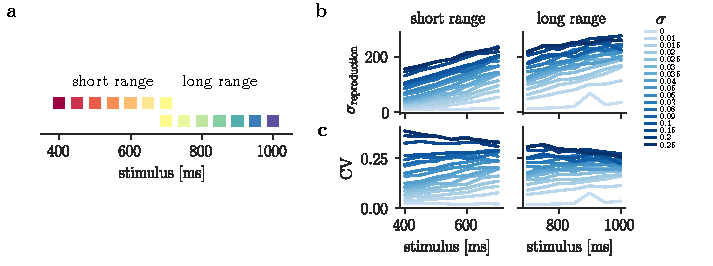
\includegraphics{figures/supp_CV.pdf}
	\caption{\textbf{Experiment description and noise levels.} 
	\textbf{(a)} The short and the long stimulus range comprised time intervals from 400 to 700 ms and 700 to 1000 ms, respectively.
	\textbf{(b)} Standard deviation of reproductions for each stimulus in an experiment simulation with 500 trials and $\tau=100$. $K$ was set to 8.5 and 6 for the short and long range respectively.
	\textbf{(c)} Same as (a) but standard deviation of reproductions normalized by stimulus duration (CV). For a noise level of $\sigma$ = 0.02, the mean CV was 0.1 for the short range and 0.15 for the long range.
	}
\label{sup:CV}
\end{figure}

\begin{figure}[!htb]
	\centering
	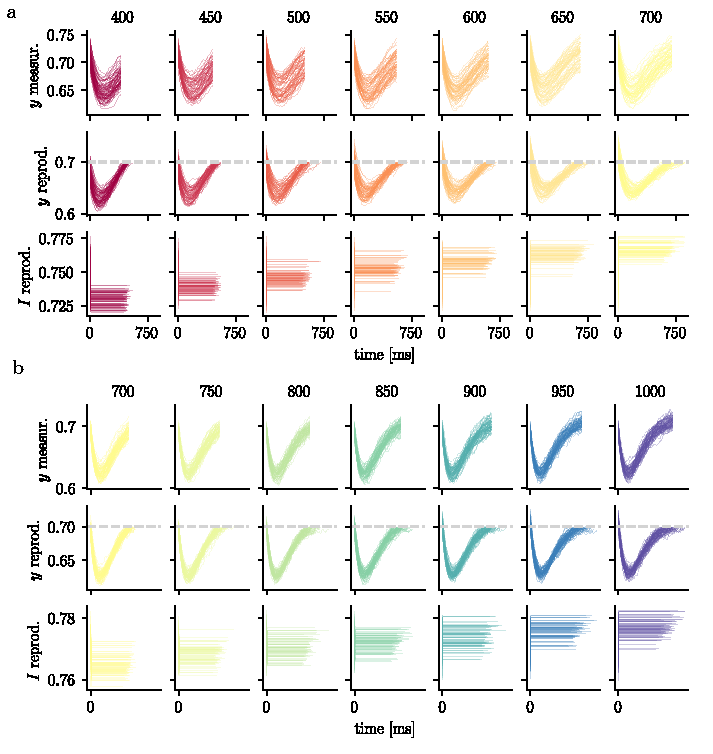
\includegraphics{figures/supp_experiment.pdf}
	\caption{\textbf{Experiment dynamics with optimized $K$.}
	\textbf{(a)} For an experiment simulation with 500 trials, a time constant $\tau$ of 130 and optimal $K = 13$, the activity was sorted according to epoch and stimulus interval. Stimuli were chosen from the short range. Upper row show the behavior of $y$ in the measurement epoch, middle row shows the behavior of $y$ in the reproduction epoch. The lower row shows the input level to the circuit during the reproduction epoch. 
	\textbf{(b)} Same as (a) with stimuli chosen from the long range and $K = 10$. 
	}
\label{sup:experiment}
\end{figure}

\begin{figure}[!htb]
	\centering
	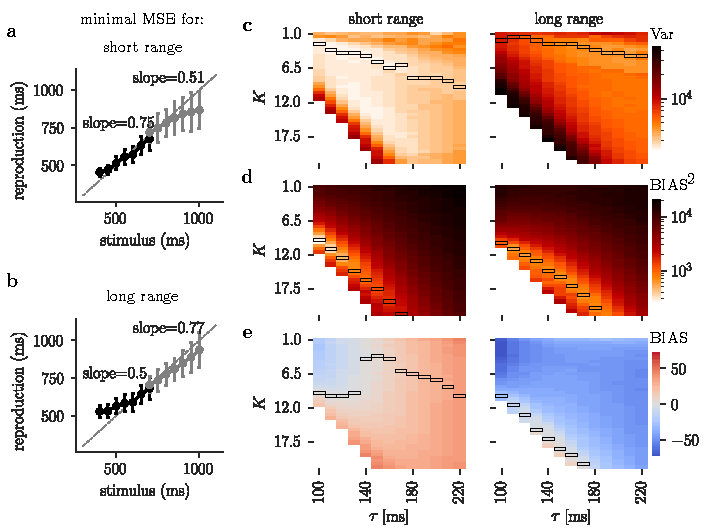
\includegraphics{figures/supp_othererror.pdf}
	\caption{\textbf{Extended parameter optimization.}
	\textbf{(a)} Behavioral results for a simulation with 500 trials, $\sigma = 0.02$ and optimized time constant $\tau$ for the short range ($\tau = 120$). For simulations with both short and long range, the optimal time constant for the short range was used. Optimal $K$ for $\tau = 120$ was 11 for the short, 7 for the long range.
	\textbf{(b)} Same as (b) with optimized $\tau$ for the long range ($\tau = 200$). Optimal $K$ for this time constant was 25 for the short range and 20 for the long range. 
	\textbf{(c)}  Simulations with 500 trials for each pair of memory parameter $K$, and $\tau$ at noise level $\sigma = 0.02$. Simulations were performed with stimuli chosen from the short (left) or long range (right). Color scale represents the variance of reproductions in the behavioral results. Minimal variance for each $\tau$ is encircled.
	\textbf{(d)} Same as (c), color scale represents the squared bias of reproductions. Minimal squared bias for each $\tau$ is encircled.
	\textbf{(e)} Same as (d), color scale represents the bias of reproductions. Values larger than 0 correspond to an overestimation, values smaller than 0 to an underestimation of the stimulus interval. Bias closest to 0 for each $\tau$ is encircled.
	}
\label{sup:othererror}
\end{figure}


\begin{figure}[!htb]
	\centering
	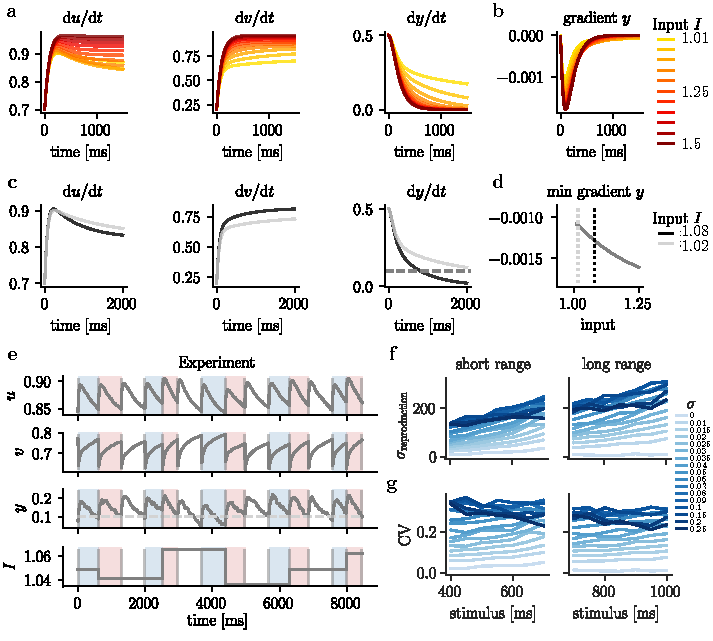
\includegraphics{figures/supp_highI.pdf}
	\caption{\textbf{Experiment description and parameter optimization in the high input regime.} 
	\textbf{(a)} Evaluation of noise for the high input regime of the model. Standard deviation (upper) and CV (lower) of reproductions for each stimulus in an experiment simulation with 500 trials and $\tau = 70$. K was set to 6 and 4 for the short and long range, respectively.
	\textbf{(b)} Simulations with 500 trials for each pair of memory parameter $K$ and time constant $\tau$ at noise level $\sigma$ = 0.02. Simulations were performed with stimuli chosen from the short (left) or long range (right). Color scale represents the slope of the linear fit between stimuli and reproductions. Behaviorally plausible slopes are encircled in blue and lie around 0.83 for the short and 0.73 for the long range. Empty spaces show simulations, that exceeded the number of timeout trials and where thus excluded from analysis.
	\textbf{(c)} Optimization of the memory parameter $K$ in the high input regime for different time constants $\tau$ at noise level $\sigma$ = 0.02. Color scale represents the MSE for an experiment stimulation with 500 trials for each pair of $K$ and $\tau$. Stimuli were either chosen from the short (left) or the long stimulus range. The minimal error for each $\tau$ is encircled in black and minimal error across all $\tau$ is additionally crossed. Parameter combinations that result in behavioral plausible slopes (b) are shaded in blue. 
	}
\label{sup:highI}
\end{figure}

\begin{figure}[!htb]
	\centering
	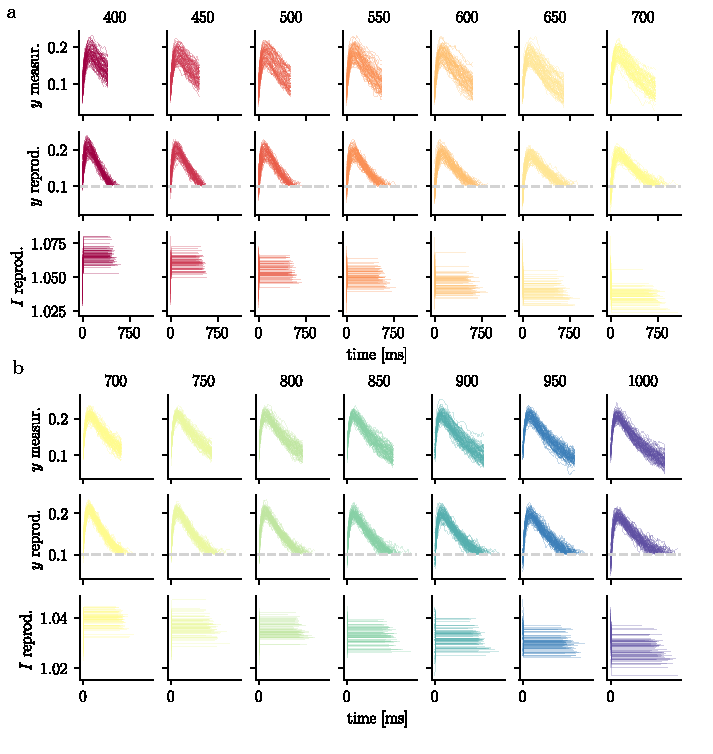
\includegraphics{figures/supp_experiment_high.pdf}
	\caption{\textbf{Experiment dynamics in the high input regime.} 
	\textbf{(a)} For an experiment simulation with 500 trials in the high input regime. The threshold is set to $y_{\text{th}}=0.1$ and $\sigma=0.02$. Parameters are set to optimized values with time constant $\tau = 60$~ms and $K = 4$. The activity was sorted according to epoch and stimulus interval. Stimuli were chosen from the short range. Upper row show the behavior of $y$ in the measurement epoch, middle row shows the behavior of $y$ in the reproduction epoch. The lower row shows the input level to the circuit during the reproduction epoch. 
	\textbf{(b)} Same as (a) with stimuli chosen from the long range and $K = 2.5$.
	}
\label{sup:experiment_high}
\end{figure}

\begin{figure}[!htb]
	\centering
	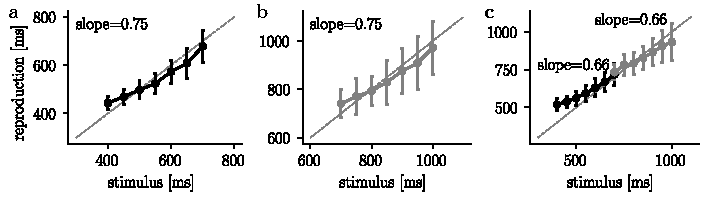
\includegraphics{figures/supp_delay.pdf}
	\caption{\textbf{Behavioral results with different delay periods.}
	\textbf{(a)} Behavioral results of an experiment simulation with stimuli of the short range and the delay period set to the mean of short range (550 ms). Time constant and update parameter are optimized based by minimizing the MSE ($\tau$ = 130, $K$ = 13). Other parameters like $\sigma$, threshold and initial values were not changed compared to previous simulations.
	\textbf{(b)} Same as (a) but for the long range with the delay period set to mean of the long range (850 ms). Optimized $\tau$ = 220 and $K$ = 22.
	\textbf{(c)} Behavioral results of experiment simulation with both the long and the short range and the delay period set to 1000 ms. The time constant is set 160 ms, which corresponds to the mean of the optimal $\tau$ for the short (110 ms) and long (210 ms) range. Optimal $K$ for the short ($K$ = 17) and long ($K$ = 11) range is optimized for the chosen time constant. 
	}
\label{sup:delay}
\end{figure}

\begin{figure}[!htb]
	\centering
	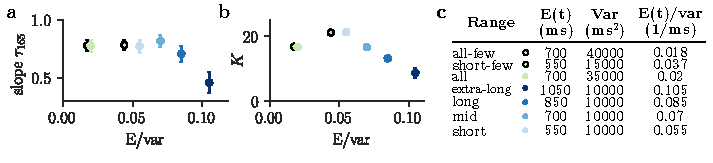
\includegraphics{figures/supp_ranges_new.pdf}
	\caption{\textbf{Influence of external variability on behavior with shared time constant.}
	\textbf{(a)} The slope of behavior resulting from experiment simulations with optimized $K$ for different ranges was determined and plotted against the ratio of mean and variance of the stimulus range. The time constant was set to 165~ms for all ranges, which corresponds to the mean of the optimal time constant of the short and long range. The error bars indicate standard deviation in the slope for different initialization. Colors correspond to the legend in (c). 
	\textbf{(b)} $K$ that minimized errors for a time constant of 165 ms for all ranges. 
	$K$ is plotted against the ratio mean and the variance of the stimulus range.
	The error bars indicate standard deviation in the slope for different initialization. 
	\textbf{(c)} Overview of all ranges used for simulations with their mean, variance and the ratio of both, that is used to characterize the ranges.
	}
\label{sup:ranges}
\end{figure}

\begin{figure}[!htb]
	\centering
	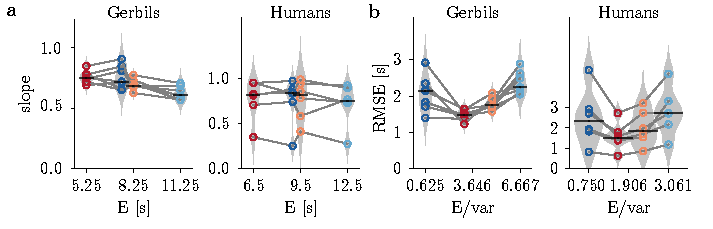
\includegraphics{figures/supp_underestimationE.pdf}
	\caption{\textbf{Effects of stimuli statistics on behavior of gerbils and humans.}
	\textbf{(a)} Slope of the linear regression between stimuli and reproductions for seven gerbils (left) and six humans (right) plotted against the mean of the stimulus ranges. Vertical black markers indicate the median of slopes and gray violin plots illustrate the distribution over all animals. Slopes for different stimulus ranges of one animal are connected by lines. Note that ranges short (red), mid (orange), long (light blue) and all (blue) differed slightly between experiments with gerbils and humans.
	\textbf{(b)} xxx
	Figure courtesy of Kay Thurley and Josephine Henke.
	}
\label{sup:underestimation}
\end{figure}

\pagebreak

\section*{Code}
\todo{I think the code design and programming stuff belongs probably to Method section}
\subsection*{Design}
The code is designed in a modular way, such that multiple types of experimental procedures with shared functionality are accessing the same basic circuit, which is implemented in \texttt{BaseSimulation} as shown in Figure \ref{fig:code}.
The implementation of the basic circuit can be reused for all epochs.
Different experiments can have different result types, all of which can be found in \texttt{result.py}. After each experiment, the results are gathered and stored together, consisting of the parameter set, the simulation time course, a list of reset time points, a list of production times, a list of indices of timeout trials and the stimulus list.
Analysis of the results is performed in the same file. Depending on the analysis (e.g. behavioral), different plots are implemented in \texttt{plot.py} to visualize the results. 

All parameters are set and described in \texttt{Params} and can be modified individually or by reading a parameter dictionary. The parameters configure the circuit. 
To initiate a simulation, the parameter set is handed to one of the implemented experiments. 
An interval reproduction experiment, as described in this report is implemented in \texttt{experiment\_simulation.py}. 
Parallel simulations of one trial (one delay, measurement and reproduction epoch) are implemented in \texttt{parallel\_simulation.py}.
Both \texttt{experiment\_simulation.py} and \texttt{parallel\_simulation.py} contain a simulate function that accesses the base simulation (\texttt{BaseSimulation}) with the implementation of the basic circuit.
For each epoch or update/reset step, the \texttt{simulate} function feeds the according time steps and initial conditions into the network in \texttt{BaseSimulation}. Depending on the epoch, the reset and update mechanism are tuned on or off. 
After each epoch or pulse, the results of the network are joint to the time course of the experiment in \texttt{trial\_update}. The \texttt{simulate} function returns a \texttt{SimulationResult} or \texttt{RangeParallelSimulationResult} object.

For an overview of the code structure see Figure \ref{fig:code} and for its usage see simulations.ipynb at \href{https://github.com/KatharinaBracher/MScThesis}{github.com/KatharinaBracher/MScThesis}. 

\subsection*{Implementation}
All simulations and analysis were performed with Python 3.9.7. 
The following libraries were used: matplotlib (3.5.1), NumPy (1.22.3), SciPy (1.8.0), scikit-learn (1.0.2). 
An experiment simulation can not be parallelized, since each step depends on the previous one.
% For the parameter search multiple experiment simulations were parallelized 

% server

\begin{figure}[ht]
	\vspace*{-2cm}
	\makebox[\textwidth][c]{\includegraphics[width=1.2\textwidth]{figures/codeStructure.drawio.pdf}}
	\caption{\textbf{Design.} The base simulation and different procedures (experiment, parallel) are all implemented in separate files. All results and analysis are collected in \texttt{result.py}, all plot for different result types are collected in \texttt{plot.py}}
\label{fig:code}
\end{figure}


\clearpage
\addcontentsline{toc}{section}{References}
\printbibliography




































\end{document}